
\documentclass[sigconf]{acmart}
\usepackage{tcolorbox}
\usepackage{xcolor}
\usepackage{colortbl}
%\usepackage{graphicx}
\usepackage{listings}
\usepackage{xcolor}

%New colors defined below
\definecolor{codegreen}{rgb}{0,0.6,0}
\definecolor{codegray}{rgb}{0.5,0.5,0.5}
\definecolor{codepurple}{rgb}{0.58,0,0.82}
\definecolor{backcolour}{rgb}{0.95,0.95,0.92}


%Code listing style named "mystyle"
\lstdefinestyle{mystyle}{
  xleftmargin=\parindent,
  backgroundcolor=\color{backcolour},   commentstyle=\color{codegreen},
  keywordstyle=\color{magenta},
  numberstyle=\tiny\color{codegray},
  stringstyle=\color{codepurple},
  basicstyle=\ttfamily\footnotesize,
  breakatwhitespace=false,         
  breaklines=true,                 
  captionpos=b,                    
  keepspaces=true,                 
  numbers=left,                    
  numbersep=5pt,                  
  showspaces=false,                
  showstringspaces=false,
  showtabs=false,                  
  tabsize=2
}

%"mystyle" code listing set
\lstset{style=mystyle}


%\usepackage{cite}
\newtcolorbox{mybox}{top=1pt,bottom=1pt,left=1pt,right=1pt,colback = white,boxrule = 0.3mm,arc = 0mm}
\definecolor{mygray}{gray}{.9}
\def\BibTeX{{\rm B\kern-.05em{\sc i\kern-.025em b}\kern-.08em
    T\kern-.1667em\lower.7ex\hbox{E}\kern-.125emX}}


\AtBeginDocument{%
  \providecommand\BibTeX{{%
    \normalfont B\kern-0.5em{\scshape i\kern-0.25em b}\kern-0.8em\TeX}}}


\setcopyright{acmcopyright}
\copyrightyear{2018}
\acmYear{2018}
\acmDOI{10.1145/1122445.1122456}


\acmConference[Internetware '20]{Woodstock '18: ACM Symposium on Neural
  Gaze Detection}{NOV 01--03, 2020}{Singapore}
\acmBooktitle{Woodstock '18: ACM Symposium on Neural Gaze Detection,
  June 03--05, 2018, Woodstock, NY}
\acmPrice{15.00}
\acmISBN{978-1-4503-XXXX-X/18/06}



\begin{document}


\title[Exploring the Dependency Network of Docker Containers]{Exploring the Dependency Network of Docker Containers: Structure, 
Diversity, and Relationship}

%Overviewing, Summerizing


\orcid{1234-5678-9012}
\author{Yinyuan Zhang*}
\affiliation{%
  \institution{National University of Defense
Technology, China}
}
\email{yinyuanzhang@nudt.edu.cn}

\author{Yang Zhang*}
\affiliation{%
  \institution{National University of Defense
Technology, China}
}
\email{yangzhang15@nudt.edu.cn}

\author{Yiwen Wu}
\affiliation{%
  \institution{National University of Defense
Technology, China}
}
\email{wuyiwen14@nudt.edu.cn}

\author{Yao Lu}
\affiliation{%
  \institution{National University of Defense
Technology, China}
}
\email{luyao08@nudt.edu.cn}

\author{Tao Wang}
\affiliation{%
  \institution{National University of Defense
Technology, China}
}
\email{taowang2005@nudt.edu.cn}

\author{Xinjun Mao}
\authornotemark[2]
\affiliation{%
  \institution{National University of Defense
Technology, China}
}
\email{xjmao@nudt.edu.cn}

\thanks{*Both are first authors and contributed equally to this work.\\
$\dag$Xinjun Mao is the corresponding author.}

\renewcommand{\shortauthors}{Yinyuan Zhang and Yang Zhang, et al.}


\begin{abstract}
Container technologies are being widely used in large scale production cloud environments, of which Docker has become the de-facto industry standard.
As a key step, containers need to define their dependent base image, which makes complex dependencies exist in a large number of containers. 
%Docker containers are not developed isolated. Instruction parameters inside dockfiles executing docker containers generation links the docker containers strongly. 
Prior studies have shown that references between software packages could form technical dependencies, thus forming a dependency network. %docker containers promote.......
However, little is known about the details of docker container dependency networks. %these studies did not explore the interconnection and development between containers. 
In this paper, we perform an empirical study on the dependency network of docker containers from more than 120,000 dockerfiles. We construct the container dependency network and analyze its network structure. Further, we focus on the Top-100 dominant containers and investigate their subnetworks, including diversity and relationships. Our findings help
to characterize and understand the container dependencies in the docker community and motivate
the need for developing container dependency management tools.

%contibute to a method of constructing dependency network of docker containers from a large-scale dockerfiles. 
%We find that most dockr containers are centered around one container and furthermore identify these influential containers. We establish the subnetwork of influential containers and analyse their network structure. The most influencial docker containers characters as Operating system and Programing language pushed the develpoment of software development together. We furthermore explore the inner causes of interconnected subnetworks and find that the interconnected closely subnetworks contribute to development of software.
\end{abstract}


\begin{CCSXML}
<ccs2012>
 <concept>
  <concept_id>10010520.10010553.10010562</concept_id>
  <concept_desc>Computer systems organization~Embedded systems</concept_desc>
  <concept_significance>500</concept_significance>
 </concept>
 <concept>
  <concept_id>10003033.10003083.10003095</concept_id>
  <concept_desc>Networks~Network reliability</concept_desc>
  <concept_significance>100</concept_significance>
 </concept>
</ccs2012>
\end{CCSXML}

\ccsdesc[500]{Software and its engineering~Software development techniques}
%\ccsdesc[300]{Computer systems organization~Redundancy}
%\ccsdesc{Computer systems organization~Robotics}
\ccsdesc[100]{Networks~Network reliability}


\keywords{Docker container, Dependency network, Network analysis}



\maketitle

\section{Introduction}
Docker is one of the most popular containerization tools in
current DevOps practice. It enables the encapsulation of software packages into containers and can run on any system~\cite{anderson2015docker}.
Since its inception in 2013, docker containers have gained 5M+
users and have been downloaded 130B+ times\footnote{https://www.docker.com/company, as of August 2020.}.  
%The ``Annual
%Container Adoption'' report\footnote{https://portworx.com/2017-container-adoption-survey/} found that 79\% of companies chose docker as their primary container technology. 
The contents of a docker container are defined by declarations
in the \textsf{dockerfile}~\cite{boettiger2015introduction} which specifies the docker commands
and the order of their execution.  
In practice, every docker container starts from a base image, which has an important effect on the container development and application~\cite{zhang2018one}; it is not uncommon to find containers in docker community depending on other containers, thereby forming complex dependency relationships.  
Thus, studying docker container dependency is
very relevant to the docker-based software development.

%With the popularity of DevOps driven by real efficiency in developing software system, an increasing amount of attention is being placed on Container, such as Docker charactering as lightweight virtualization technology to deploy software infrastructure. Docker containers defined by Dockerfile's declarative instructions package an application with its dependencies execution environment and function as running Docker Contaier.

On the one hand, with the widespread use and influence of docker, many
studies have been recently conducted to investigate the dockerfile usage practices~\cite{cito2017empirical,zhang2019clustering,henkel2020mining}. Those works have emerged a lot of great findings and brought many practical implications
to developers, but are not designed to look into the details
of docker container dependency. 
The management practices of container dependency have received little
attention, despite being a crucial part of almost all docker projects. 
On the other hand, prior studies~\cite{blincoe2015ecosystems,decan2016topology} have shown that references between software packages could form technical dependencies, thus forming a dependency network. Recently, network-based analysis of programming language dependency networks has emerged, and many studies have analyzed the topologies of npm, PyPI, CRAN, and Rails~\cite{wittern2016look,decan2016topology,zhang2018within}. 
However, there is still a lack of early exploration of the docker container dependency network.

%As software system grows in scale and complexity,so does Docker. The research on growth of docker containers whose content defined completely by dockerfile can be done through the research of prasing dockerfiles. Mining potential link or knowledge of docker containers with their scale expanding regularly would be valuable. Previous studies focuxes on optimization of docker configuration or the fast and high quality build of dockerfiles, however, rarely mentioned the relationship and knowledge between docker containers.......
 
%Given the ubiquitous nature in industry, we study the inter connection between docker containers, especially those core containers brought strong appeal and cohesion. The "FROM" instruction defined by docker rule decide the reliable relationships between a pair of docker container. Furturemore, docker containers mostly built from other base container can also function as other directed base container which depends the interconnetd relationships between docker containers. Based on the above ubiquitous relationships nature, we gain the strong dependency relationships and future explore the dependency character through network mertics. 

%We conduct an exploratory empirical study with the goal of charactering the dependency network between docker containers and capturing the interconnected relationships and analysing the inter connection causes between subnetworks centraled by influencial containers.
In this work, we take a novel network-based approach
for studying dependency networks of docker containers. We use data from more than 120,000 dockerfiles in a public dataset. We compose network of containers based
on dependency relations to understand what the static properties and topologies of docker container dependency networks and what the differences and relationships between internal subnetworks.

The goal of this work is to study the state of current
dependency network of docker containers, to understand their structure, and to characterize their diversity and coupling relationship. We have formulated the
following research themes to guide our research:

\textsf{RT1}: \emph{What are the characteristics of docker container dependency network?} (see Section~\ref{sec:rt1})

\textsf{RT2}: \emph{How diversified and coupled are the containers in the docker container dependency network?} (see Section~\ref{sec:rt2})

Answers to these questions can help to quantify the state of
the docker container ecosystems, give an overview of the trends in container dependency management, and can inform the development of improved dependency management tools. 
In summary, this work has three core contributions:% through our exploratory study:
%The highlights of our quantitative findings are: 



\begin{itemize}
%\item \textbf{We conduct the first large-scale empirical study to construct and analyse dependency relationships between docker containers by network structure metric.}
%\item \textbf{We find the TOP-100 influential containers and explore the character of the subnetworks constructed by these containers}
%\item \textbf{We analyse the internal mechanism of subnetwork development and future analyse the inter causes hiddend dockerfile resulting the interactive links between subnetwork.}

\item To the best of our knowledge, we are the first to systematically investigate the docker container dependency networks, including their structure, diversity, and relationships.
\item We design automatic tools for capturing technical dependencies and constructing dependency networks of docker containers. Data and source codes can be found online\footnote{https://github.com/yinyuanzhang/container-dependency-network}.
\item Our analysis of the container dependency networks result in a series of findings and further distill some implications for different stakeholders.%We discovered and summarized three existential/dependent relationships between core docker containers.
\end{itemize}


The rest of our paper is organized as follows. Section~\ref{sec:rs} discusses the research setup. The detailed results of our study are presented in Section~\ref{sec:rt1} and Section~\ref{sec:rt2}. In Section~\ref{sec:di}, we present the discussion and discuss the related work in Section~\ref{sec:rw}. Finally, we conclude this paper in Section~\ref{sec:co}. 


%\section{records}
%and we highlight some key future research directions to improve the Ethereum ecosystem.

 %fundamental data analysis task

%Overview and Analysis of Docker container Dependency Network: Structure, Diversity, and Link Paradigm


\section{Research Setup}
\label{sec:rs}
%To support quantitative studies on RQs, we perform dataset processing and constructing container Dependency Network.
To perform our study, we first define the dependency network of docker containers. Then, we present our dataset and tools, and discuss our research questions.

\subsection{Dependency Network of Docker Containers}
\label{subsec:cdn}
In docker containers, dockerfile is a text document that contains all
the commands a user could call on the command line to assemble an image~\cite{zhang2019clustering}. 
The instructions stored in dockerfiles define naturally the 
content of docker containers, including the application, 
dependencies along with the execution environment. 
Especially, following the official dockerfile best 
practice\footnote{ https://www.docker.com/blog/intro-guide-to-dockerfile-best-practices/}, 
a valid dockerfile must start with a \texttt{FROM} instruction where one container inherits 
infrastructure definitions from another container, e.g., \emph{FROM ubuntu}. The reference relationships 
captured by \texttt{FROM} instruction thus can be regarded as technical dependency between docker containers. 


Specifically, we call container that has \texttt{FROM} instruction pointing to another container as \emph{Source container}, and container that is pointed to from another container's \texttt{FROM} instruction as \emph{Target container}. We say that a pair of containers, C$_i$ and C$_j$, are a \emph{container pair}, (C$_i$, C$_j$), if the \texttt{FROM} instruction of container C$_i$ points to C$_j$. As showed in Listing 1, in the container Tomcat, \texttt{FROM} instruction defines the base container as \emph{ubuntu:16.04}, thus can be identified as a container pair (\emph{Tomcat, Ubuntu}), i.e., Tomcat$\rightarrow$Ubuntu.



\begin{lstlisting}[caption= An example of Dockerfile of container Tomcat]
FROM ubuntu:16.04  

ADD ["startup.sh", "."]  
  
ENTRYPOINT ["./startup.sh"]  
\end{lstlisting}

Based on those container pairs, we further construct the integral dependency network of docker containers. The \emph{Container Dependency Network}, referenced to Jurgen et al.'s research \cite{blincoe2015ecosystems}, is defined as a directed network \emph{N} = $\left \langle V,E \right \rangle$. The set of vertices, denoted by \emph{V}, is all docker containers. The set of edges, denoted by \emph{E}, indicating the container pairs \emph{E(V)} = $\left\{ 	\left( Ci, Cj \right)|Ci,Cj \in V \right\}$. %If the container represented by node x$_i$ instruction link the container represented by node y$_j$. 
Note that we also mark the weight of each edge $E_{ij}$, 
which is computed as the number of container pairs ($C_i$,$C_j$) created in history. 
The weight can characterize the frequency of the historical usage of the container pair. 
For example, if we find three Dockerfiles in our dataset contain the ($C_i$,$C_j$), the weight of $E_{ij}$ is 3.\\




\subsection{Dataset and Tools}

%We first see the containers with different versions have almost similar function and futher ignore the container tag to reveal more actural dependency relationships.(e.g.. ubuntu and ubuntu3.6) We then remove  owner of containers based on the hypothesis that different private owner create containers with the same name to play a similar role in real usage environment.
Our initial dataset comes from public Kaggle dataset\footnote{https://www.kaggle.com/stanfordcompute/dockerfiles/version/1}, 
which contains 129,463 dockerfiles extracted in early summer 2018. 
Based on those dockerfiles, we extract all \emph{container pairs} and construct the dependency network, as shown in Figure~\ref{fig:process}.    %129,463
Specifically, there are five steps: 
\begin{figure}[h!]
\centering
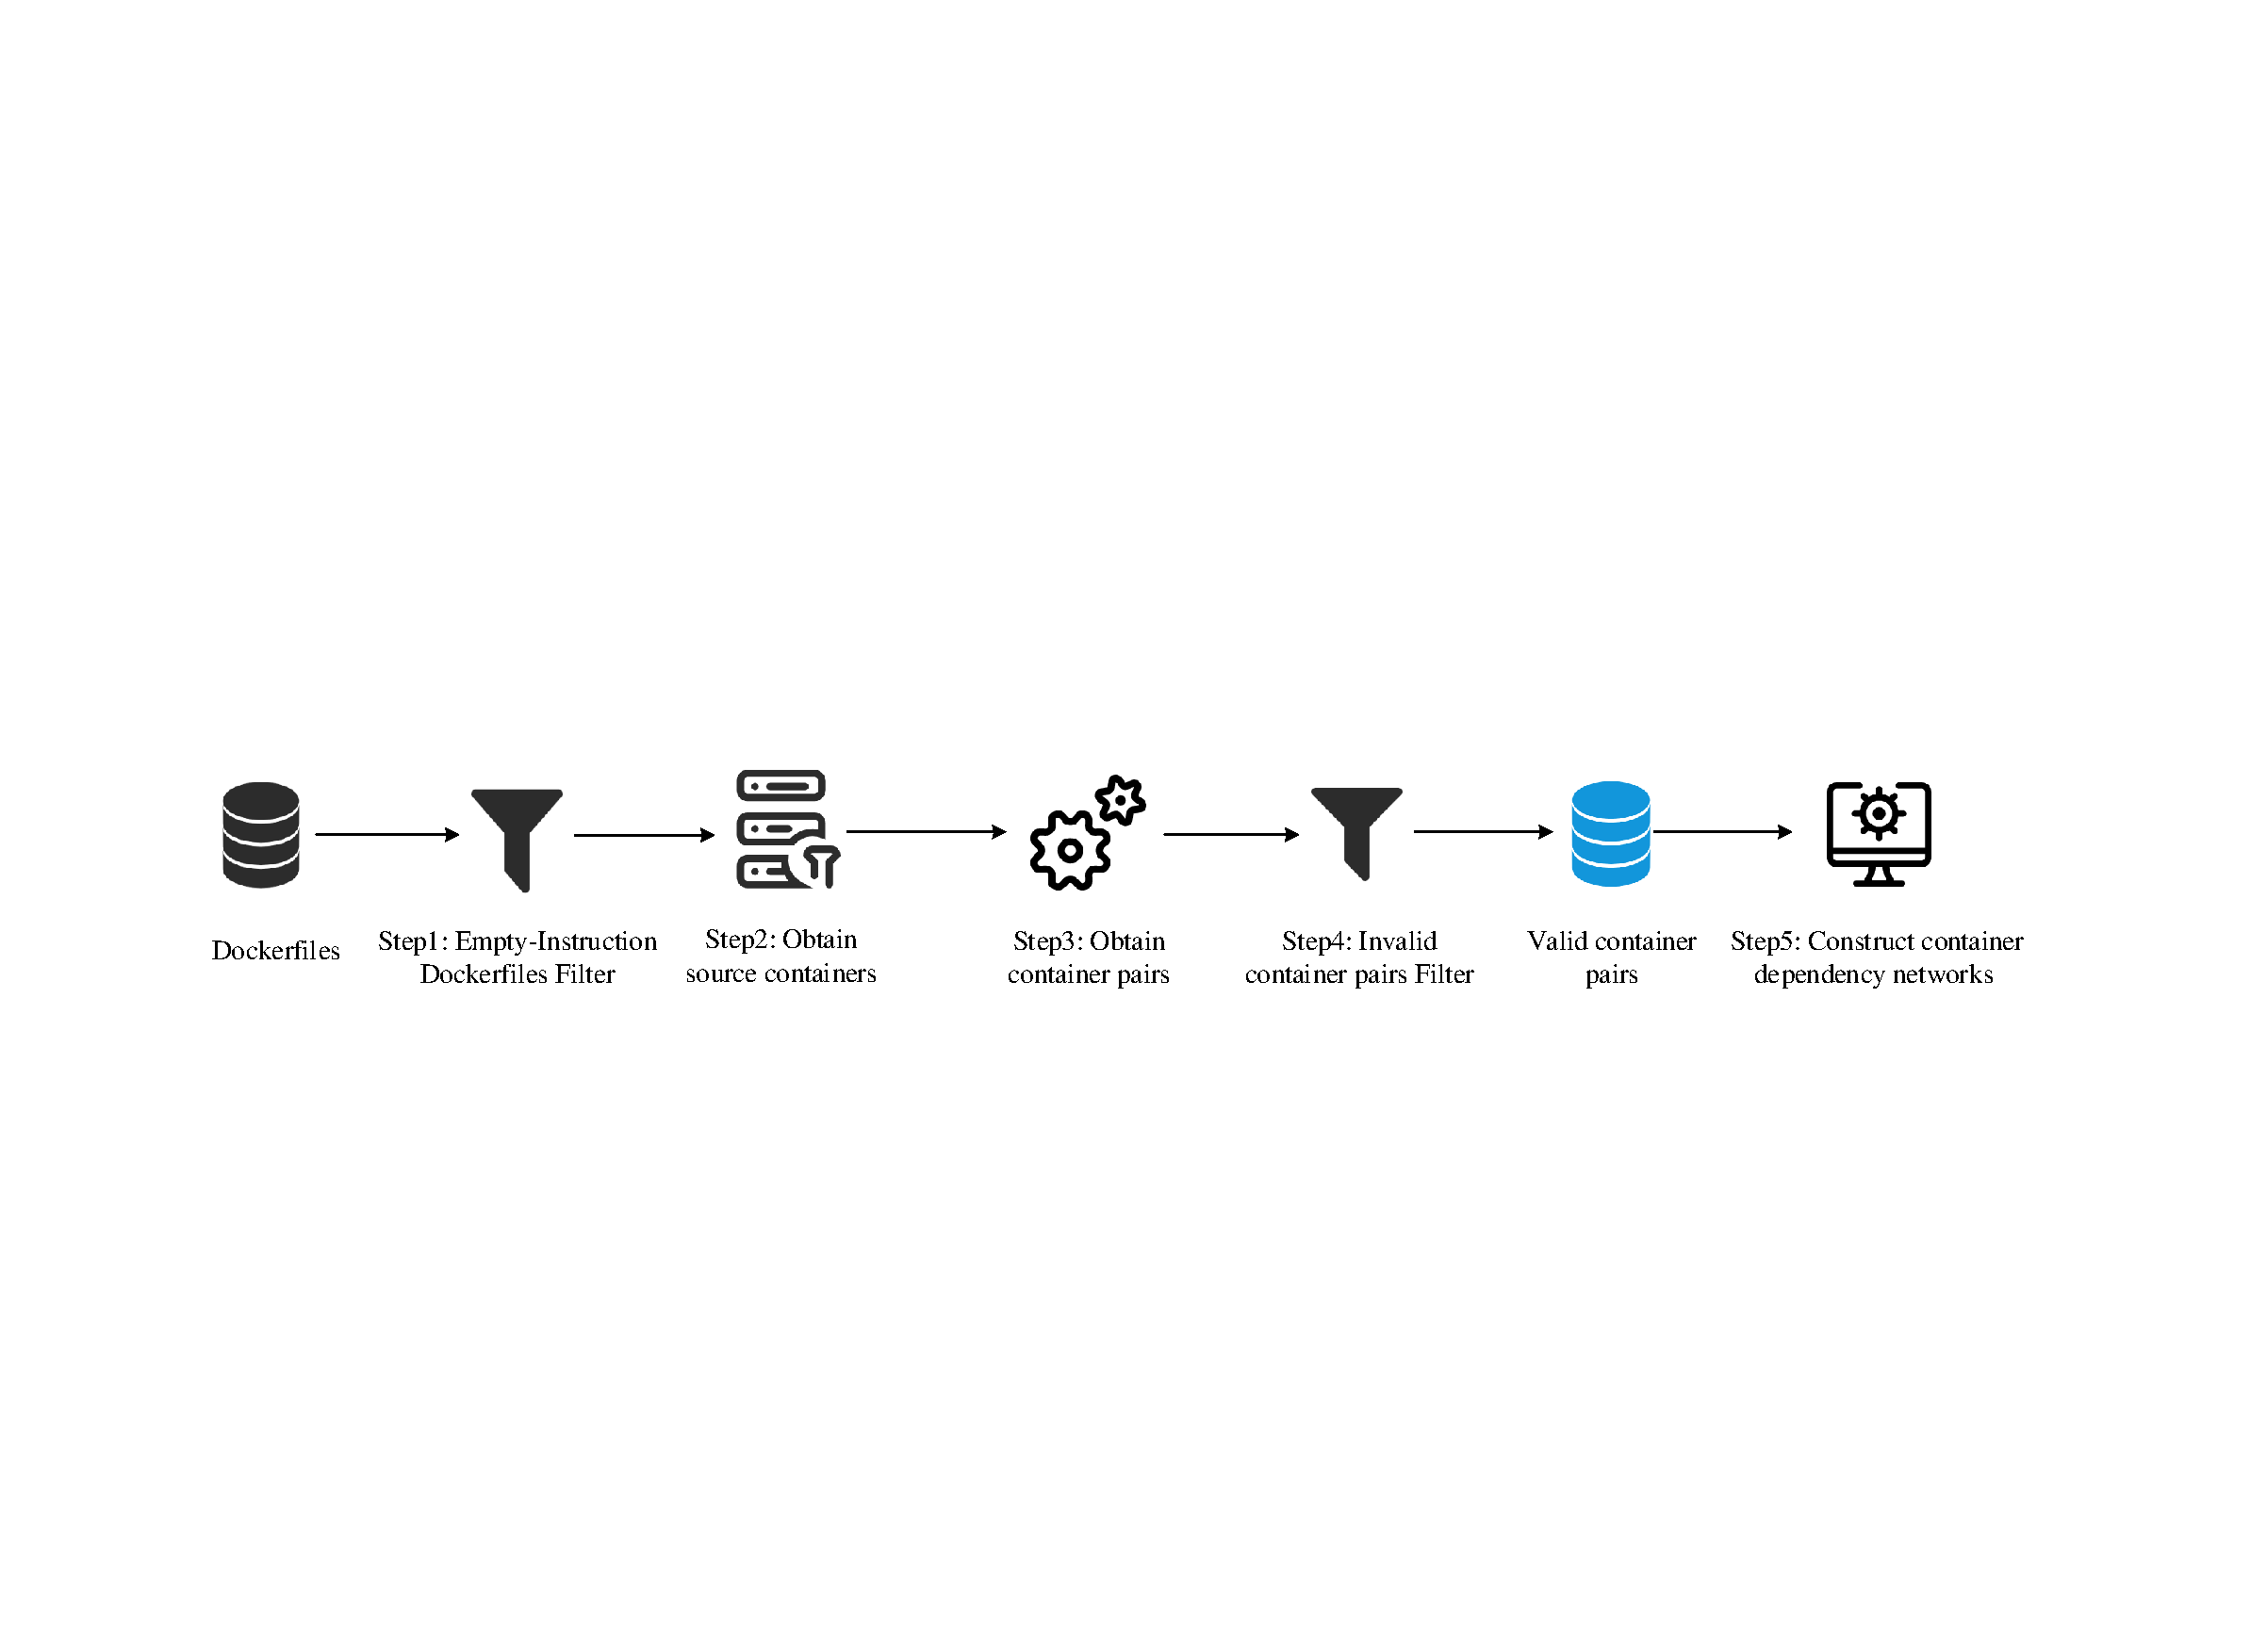
\includegraphics[width=1\columnwidth]{picture/Dataset_process3.pdf}\vspace{-0.3cm}
\caption{Overview of our data preprocess.}\vspace{-0.3cm}
\label{fig:process}
\end{figure}



\noindent\textbf{Step1: Removing dockerfiles with empty FROM instruction}. We find that FROM instructions were not correctly defined in many dockerfiles, e.g., missing FROM instruction or base container parameter. %The dockerfiles with empty FROM instruction that provide infrastructure for building containers were first removed. 
%As the study of Yiwen et al. points out that dockerfile lacking infrastructure can be considered as a low-quality build script, which is always prone to build failure in practice. 
To eliminate the threat, we remove those dockerfiles with empty FROM instruction; this yields 128,247 valid dockerfiles.
%To filter the empty instruction dockerfiles, we determined whether is \emph{FROM instruction} dockerfile by parsing each dockerfile and got 128,247 available dockerfiles. 

%After preliminary filtration of empty-instruction dockerfiles, we obtained 128,247 available dockerfiles.      %128,247  

\noindent\textbf{Step2: Obtaining source containers}. In the Kaggle dockerfile dataset, dockerfiles are stored in folders, with the catalog information being \emph{owner/repository/dockerfile}. 
Thus, we extract the repository name from each dockerfile and find 82,188 unique source containers. 
%removed the owner describing container creator personal information and captured repository information identified as the Source container id.   


\noindent\textbf{Step3: Obtaining container pairs}.  
Firstly, we capture the base container information by extracting its name from the specification in FROM instruction, i.e., a tuple of the form \emph{namespace/name(:version)}; This yields 9,270 target container names. 
Note that we 
%\emph\noindent\textbf{geting available parsing parameters:} This producer aims at praising and capturing available parameters content by 
ignore the FROM instruction following with "\#" used for interpretative statement. With source containers' information, we finally obtain 130,830 container pairs.
%Next, 
%Afterwards, \emph\noindent\textbf{removing version information:} The content of parameters is manifested as the \emph{base:version} format, \emph{base} represents specific function while \emph{version} changes without changing the basic functionality(e.g.. ubuntu and ubuntu3.6). Thus, we removed the version information and further identified \emph{base} as the Target container id. % 130,830
%\noindent\textbf{Step4: Combining container pairs}. The obtained source container and target container, representing real identity information, have a consistent format. Further, we combined a source container and a target container corresponding to the same file as an container pair in the form of (source container, target container). Finally, we got 130,830 container pairs sequence. 
% 130,830

\noindent\textbf{Step4: Filtering out invalid container pairs}. We find that in those container pairs, there exist many source containers that equal to their target containers. 
Also, we find some target containers have no specific meaning, e.g., \emph{``none''}, \emph{``container''}. 
To reduce threats, We filter out those invalid container pairs.
Finally, we collect 124,384 valid container pairs for the dependency network construction.
%yeilding %considered thisour  self-reference container pair to be an invalid technical dependency and after this filter, We obtained 124,384 pairs of containers pairs with effective technology dependence. %124384-1=124383     83030 nodes  \\


\noindent\textbf{Step5: Constructing container dependency network}. First, we construct the overall dependency network based on all the container pairs. Further, we group container pairs according to their characteristics, and build the subnetworks of selected core containers. Finally, for the overall dependency network and subnetworks, we calculate their network metrics and perform the quantitative study on them.%generated visual network charts using Gephi tool. 




In order to foster reproducibility and follow-up studies, 
we provide a comprehensive reproducibility package, 
containing tool chain, database, queries and analysis scripts. 
Our dataset and additional scripts can be found online at GitHub\footnote{https://github.com/yinyuanzhang/container-dependency-network}.  
The tool chain consists of separate python projects: \textsf{dockerfile-dependency}\footnote{https://github.com/yinyuanzhang/dockerdependency} is responsible for parsing and generating container pairs, and \textsf{dockerfile-network}\footnote{https://github.com/yinyuanzhang/dockernetwork} is responsible for constructing networks and calculating network metrics.% and further create visual charts via Gephi. %We make it available together with all of our analyses on GitHub for inspection and reproduction.







\subsection{Research Question}
%Guided by the purposes of exploring the integrated structure and characteristics of docker container network, 
%To better explore the dependency network of docker containers, including its structure, diversity, and relationship, we formulate two research themes. 
Our study seeks to answer several research questions that we group into two research themes. 
The overall motivation is to analyze structure, diversity, and
relationships of docker container dependency networks to get insights into current dependency usage and possible issues. 
Next, we explain the
motivation behind each research theme in more detail. 

\smallskip
\textbf{RT1: (Structure) What are the characteristics of docker container dependency network?}  
Currently, not much is known about
the static properties and topologies of docker container dependency networks. For example, we know to what extent
dependencies are used in traditional packages only~\cite{decan2019empirical,wittern2016look}. However, we do not know if there are differences in dependency
usages across docker containers? 
In practice, developers can freely define the base image of the container; it is not uncommon to find  some containers that are dependent by a large number of other containers, while some are not.   
However, we do not know which containers are the most influential. Answers to these questions enable
us to understand the current state of container dependency networks
and would be the starting point for analyzing their  
internal characteristics. Specifically, we ask the following questions:

%The first research theme aims at understanding the structure of the overall container dependency network that leads to the core containers distribution and quantifies feature, and the second research theme aims at mining the diversity feature and relationship of subnetwork based on core containers.

% We present our study's five key RQs on the structure, diversity and revelence of docker container network, divided into two parts - 


\emph{RQ1: What does the container dependency network look like?}

\emph{RQ2: How are container dependencies distributed?}

\emph{RQ3: What are the dominant containers in the network?}


\smallskip
\textbf{RT2: (Diversity and relationship) How diversified and coupled are the containers in the docker container dependency network?} 
The dominant containers located in the central hub of the network are supposed to be important and could affect a number of other containers. As a result, those core containers and satellite containers form a variety of subnetworks. 
However, we do not know whether these subnetworks will be diversified or have significant differences. 
Moreover, due to the interconnected part of the overall network, the connections between the subnetworks are apparent, e.g., the same container in two projects depends on two different containers. However, we do not know much about the closeness / coupling between different subnetworks. 
%The core containers bringing attraction and cohesion for Docker Ecosystem prosperity deserve deeper exploration. %Furthermore, we construct and consider subnetworks from within and across dimensions:
Thus, investigation into these questions would help us to understand the diversity and relationship of container dependency networks. Such information could be incorporated in measuring container importance with regards to interconnection in the container dependency network.  
Specifically, we ask three research questions:

\emph{RQ4: What are the types of container dependency subnetworks?}

\emph{RQ5: What is the difference between subnetworks?}

\emph{RQ6: How connected are the subnetworks?}




\section{RT1: network structure}
\label{sec:rt1}
\subsection{RQ1: What does the container dependency network look like?}
%\noindent\textbf{Motivation. }The initial RQ1-1 aims at understanding the integrated network structure. Docker containers are not developed isolated,  relationships between them are built up through technological dependence with the increasing scale of docker containers ecosystem. Docker is widely used in the open-source community. Prior studies, however, focus on performance aspects and there is little research on the dependency relationship between docker containers. Thus, overviewing and computing the network structure properties will help to understand the compactness structure of the docker containers network and motivate more work on relationships of docker containers in the future.
First, we build the container dependency network based on our dataset and describe its basic network properties.

\noindent\textbf{Approach}. 
As mentioned in Section~\ref{subsec:cdn}, the container dependency network is composed of container pairs.  
To virtualize the container dependency network, we mainly use the \emph{Gephi tool}\footnote{https://gephi.org/}. 
Further, we analyze the basic network structural properties, including  
%To address RQ1-1, we primarily use network metric including 
\emph{diameter} and \emph{average shortest path}. 
 Specifically, \emph{diameter} is defined as the maximum of the length between any nodes, and \emph{average shortest path} is calculated as the average of all the length between nodes. 
%Future, we compare the technical metric of \emph{Container Dependency Network} with other networks including software projects network and social coding network.

%To future present properties of the docker containers network, we analyzed visualizations of the Dependency Network. We used the Gephi graphing tool to create visualizations.

\smallskip
\noindent\textbf{Results}. 
The container dependency network consists of 83,030 nodes and 98,248 edges. Figure~\ref{fig:full} shows the full network overview, though for visibility we only display nodes with degree of 10 or greater.
%The 128,384 container pairs sequence described in Section 2.1 generate 83,030 nodes and 98,248 edges attached with weight representing frequency times in the integrated docker containers network. 
%Figure 1 shows the integrated \emph{Container Dependency Network}, though for visibility we only display nodes with a degree of 10 or greater. 
The size of the node represents the degree of the node, while the thickness of the edge represents the weight of the edge and the color of the edge represents different modular provided by Gephi tool. 
As visible on the graph, most of the nodes depend on each other which forms huge components, but there are also some isolated nodes that are connected to only a small number of nodes. 
Furthermore, we find that the size of some nodes or some edges are larger than others, indicating that there exist some dominant nodes  in the network, and that some container pairs have been frequently used in history. 

% The reason may be that, on the one hand, ....  A potential explanation is that 
% 2578    220     124384    124384-220-2578=121586    121586-2578=119008 /121586= 97.8%
% 1216    119008-1216=117792/120370 = 97.85% 

\begin{figure}[h!]
  \centering
  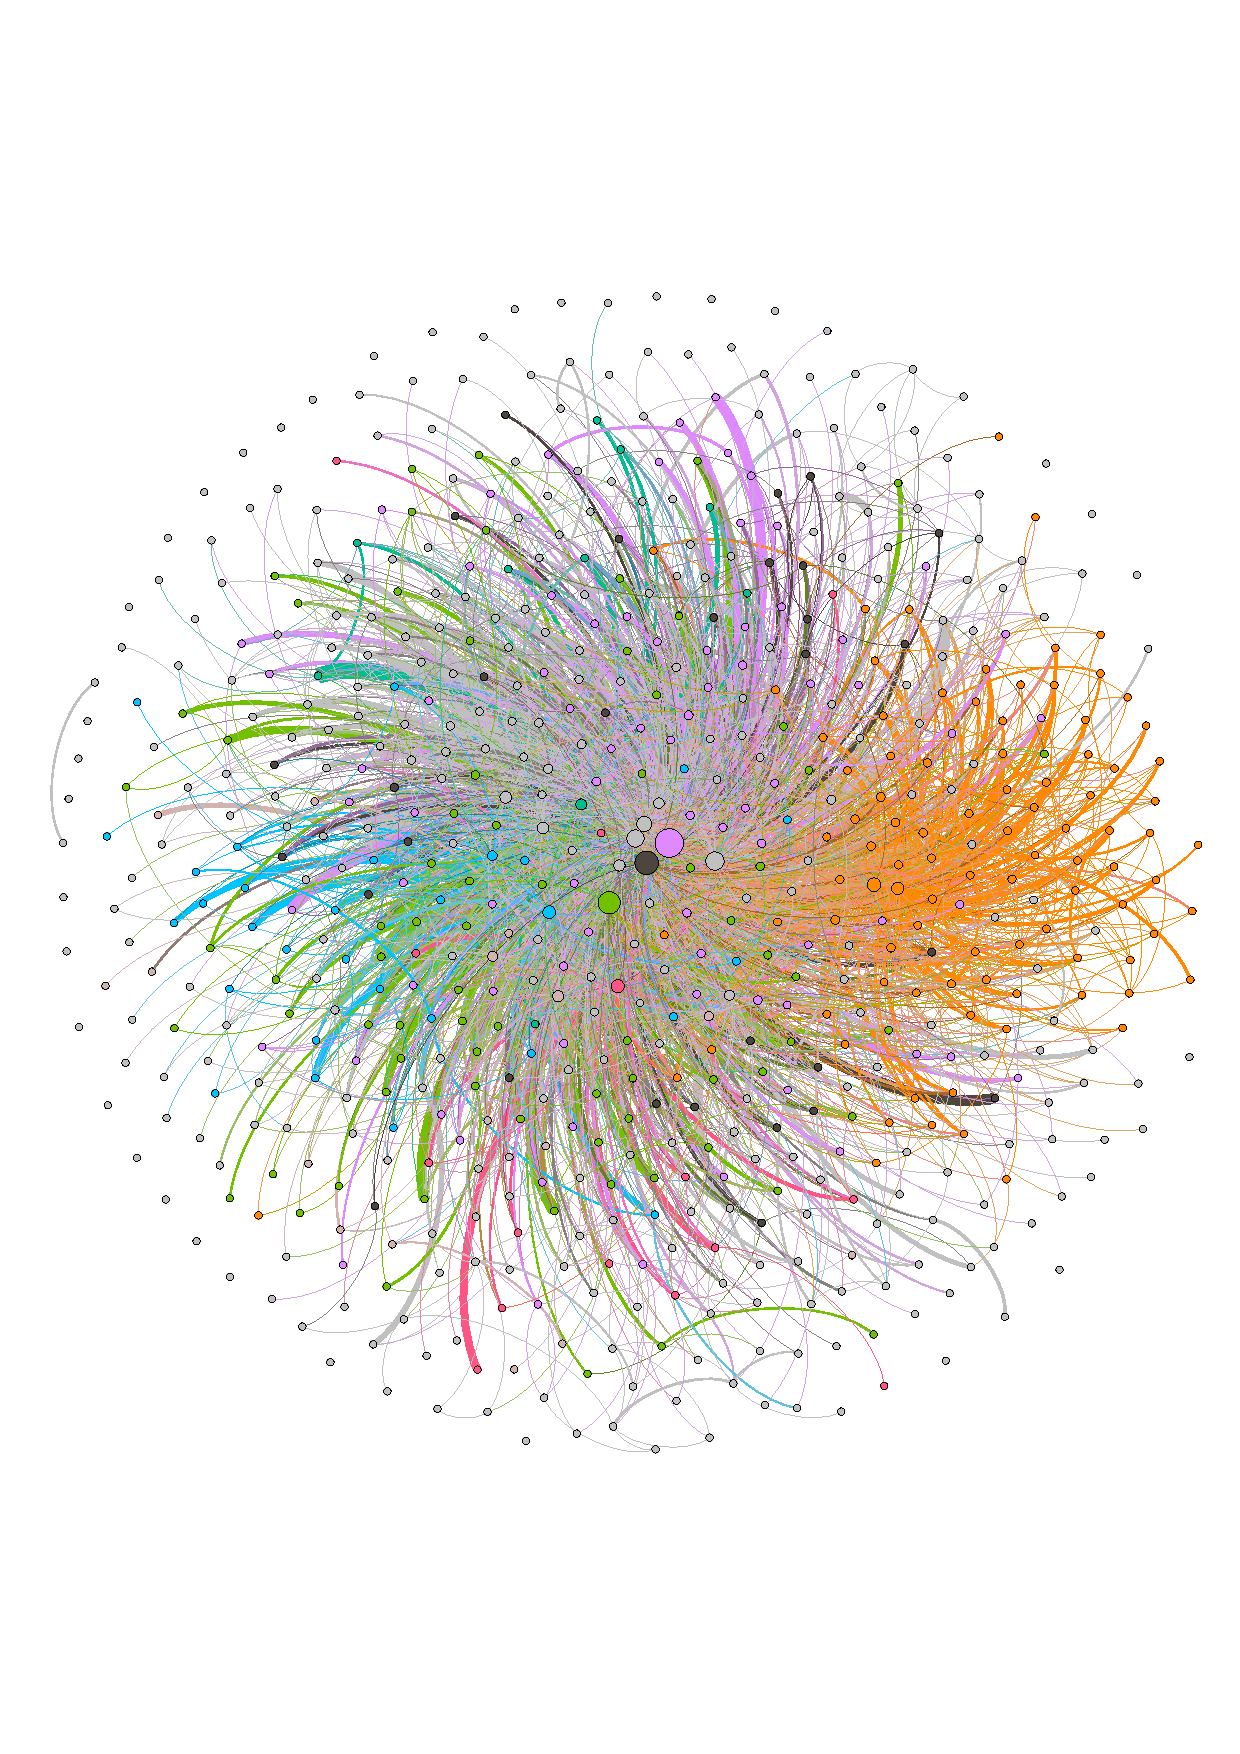
\includegraphics[width=0.97\columnwidth]{picture/overview_imagenet.pdf}\vspace{-0.3cm}  
\caption{Overview of the docker container dependency network.  Redrawn by Fruchterman Reingold algorithm.}
\label{fig:full}
\end{figure}


The \emph{diameter} computed in the container dependency network is 23 and the \emph{average shortest path} is 5.72. These numbers are larger than the findings reported for developer social networks~\cite{zhang2017social} and project relationship networks~\cite{thung2013network},   
%The average short path is 5.72, larg.
%For integrated container network, the diameter calculated is 23, as well as the average path length is 5.7173. Compared with Github projects network(diameter= , average path length=) and social coding network(diameter= , average path length=), the docker containers network feature a larger diameter and average shortest path between nodes, 
implying that container dependency networks are actually looser than other real networks. 
%the interconnection of docker containers is relatively loose.
The potential reason may be caused by the way the container establishes technical dependencies. 
In fact, 97.85\% dockerfiles in our dataset only contain one FROM instruction, most of source containers only have one target container. A small part of the dockerfiles depend on multiple base images at the same time, which may be related to their design to combine multiple microservices. 
The configuration characteristic of dockerfile may make technical dependency reliable, but it would cause the overall connectivity of the container dependency network to be very loose,
to be further explored in future work.
%Although those technical dependencies are more reliable, the interconnection between container nodes is actually not strong. 
%On the one hand, technical dependence we captured between docker containers come from \emph{FROM instruction} to inherited infrastructure definitions seems extremely reliable. The technical dependent inside the Github project network emerging from an issue or co-author, relatively, is not reliable.  On the other hand, considering the composition of internal instructions in dockerfile, the rate of single-from-instruction dockerfiles number is 97.85\% of all dockerfiles.        

\begin{mybox}
\emph{Answer to RQ1}: There are dominant containers in the container dependency network and some container pairs are widely used. However, the interconnection of the docker container dependency network is relatively loose. 
\end{mybox}






\subsection{RQ2: How are container dependencies distributed?}
%\noindent\textbf{Motivation. }The integrated network structure mentioned in Section 3.1 has reveals the interconnection between docker containers. With the diversity of Docker containers, research on the regular differences between container nodes will be important, since it helps practitioners find the potential reason to promote the prevalence of docker containers. Thus, this RQ aims to mine the distribution feature of docker containers to further explore the distribution difference between docker containers. 
Next, we aim to analyze the distribution of container dependencies, i.e., their node degree, among all container nodes. 

%The potential to get insights into the reason for diversity of container ecosystem motivate the exploration of container node distribution.

\noindent\textbf{Approach}. 
For each container node in the container dependency network, 
we calculate its \emph{indegree}, \emph{outdegree}, and \emph{total degree}. The \emph{indegree} is computed as the number of all the nodes point directly to the given node. The \emph{outdegree} is computed as the number of all the nodes that the given node points to. The total \emph{degree} is the sum of \emph{indegree} and \emph{outdegree}. The degree distribution represents the relative frequency of each value of the node degree in the container dependency network.

%of an container is the frequency of other containers pointing to the container, the \emph{out degree} of the container is the frequency of the container pointing to other containers, and the \emph{degree} of the container is the sum of the \emph{in degree} and the \emph{out degree} of the container.

%For given container node, high degree indicate that tight connection between it with other containers but low degree of the given container represents it is connected loosely or nearly isolated with the most nodes, showing that an optimal solution to describe the influence of container has been found.  Further, we explore the distribution about number of containers across container \emph{in degree}, \emph{out degree} and \emph{degree}. 


\begin{figure}[h!]
\centering
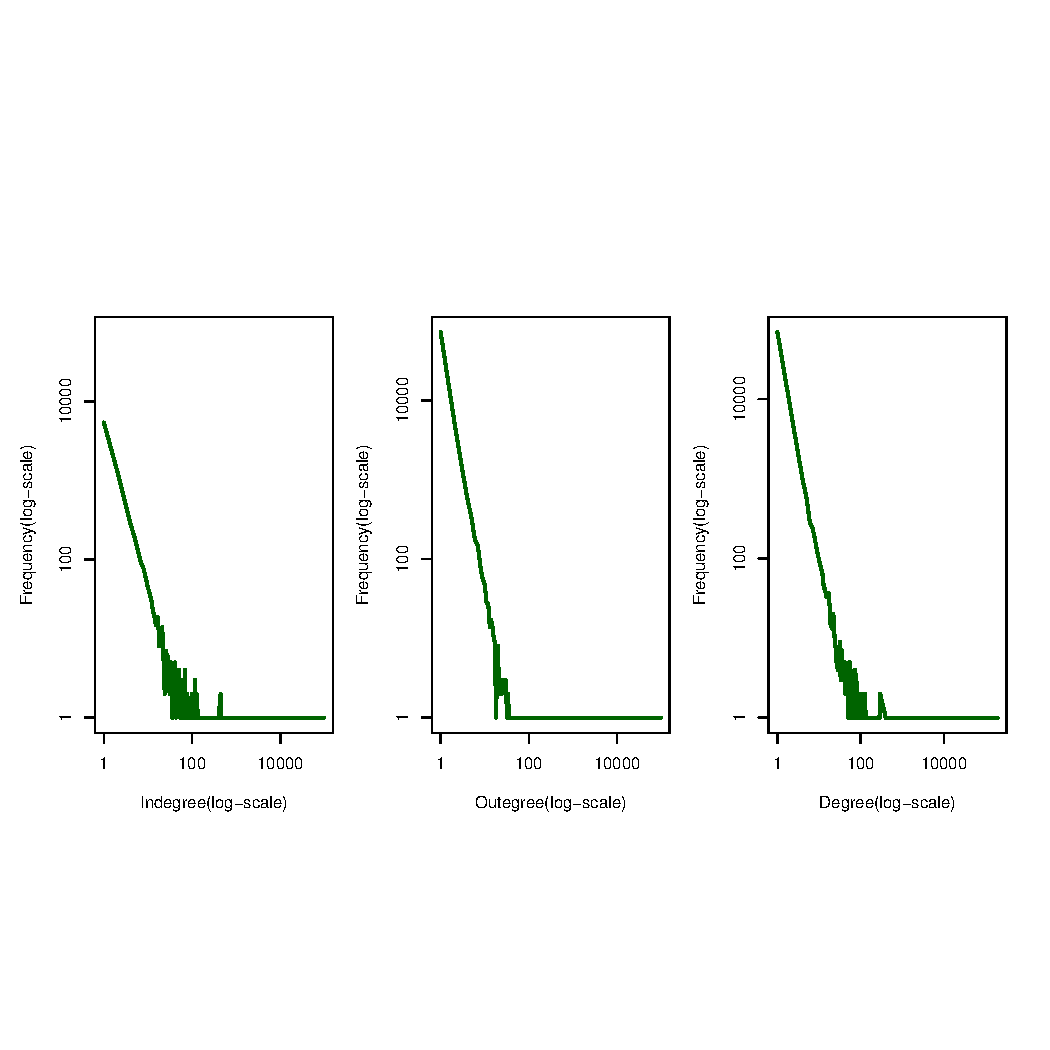
\includegraphics[width=1\columnwidth]{picture/image_distribution_degree.pdf}\vspace{-0.3cm}
\caption{Docker containers' degree distribution. y-axis shows the number of containers having given node degrees.}\vspace{-0.3cm}
\label{fig:distribution}
\end{figure}

\noindent\textbf{Results}. 
As shown in Figure~\ref{fig:distribution}, we can observe that all distributions display the power law relationship and follow a long tail distribution~\cite{anderson2007long},  
indicating that container dependency network is a scale-free network. A very small number of containers, however, may occupy a greater degree in the total network. 
The average node degree of the container dependency network is 2.36  (indegree: 1.18, outdegree: 1.18), indicating that each container may depend on 1.18 other containers and be dependent on 1.18 times. 
This is consistent with the notion that most containers only depend on only one base image. 
%The degree distribution across 83030 containers showed as figure 2 follows a typical long tail distribution, indicating that a very small number of containers, however, occupy a greater degree in integrated \emph{Docker container Network}. 
It also reveals that most containers rely on several central containers. 
%{\color{blue}{Interestingly, this finding is similar to the conclusion that the core project has a powerful appeal to open ecosystem by beida.etc.}}  A potential explanation is that 
Because using popular docker containers with strong convince is in line with most practitioners, especially for new docker users. 

In this network, a successful container may attract more containers to reference, while many containers will stagnate after a short while. The number of dependents of a container may be an important positive feedback factor in determining the influence of a container. 
However, we find that some containers depend on multiple base images. 
These containers are also linchpin nodes in the community network, who link containers together into clusters. 
Thus, for those containers that are at the tail but linking different clusters %docker containers being cohesiveness and charisma in the network 
may also play a huge and important role in the docker container development.

% talk degree eg..the number of degree=1. 




\begin{mybox}
\emph{Answer to RQ2}: 
The degree distribution of docker containers follows a typical long-tail distribution. 
Containers with a large number of dependents or linking different clusters may be important factors that affect the container community.
%indicating that very few containers, however, bring  cohesiveness and charisma for docker ecosystem.
\end{mybox}




\subsection{RQ3: What are the dominant containers in the network?}
%\noindent\textbf{Motivation. }Despite the prevalence of Docker ecosystem mainly appealed by core Docker containers, however, concerns emerge on the core docker containers and why they have strong cohesiveness for Docker ecosystem need further research. This RQ aims at identifying the core containers in detail. Knowing more information about core containers contributes to understanding their support for software development. 
In this RQ, we want to identify the most influential (i.e., dominant) containers from the container dependency network. 

\noindent\textbf{Approach}. We consider dominant containers are those containers with high degrees, because they have more connections in the container dependency network. % that indicates well-connected containers among docker ecosystem.
For each container, we compute its degree values and degree rate (node degrees/all degrees). Then, we 
range all containers in terms of the degree rate. 
Since we are most interested in studying the dominant containers, we focus our analysis on the Top-100 containers with the highest degrees. 
%Further, we ranged and investigated the TOP-100 core containers according to the degree of docker containers and further compute \emph{in degree}, \emph{out degree} and \emph{degree rate} of the core containers. This approach allows to cover significant parts of the overall data, as core containers bring prosperity to docker container ecosystem.  % represent main docker containers influence.

\noindent\textbf{Results}. 
We find that although Top-100 containers only occupy 
%For top-100 core docker containers, though, the number is only 
0.12\% of all containers, they occupy 39.90\% of all degrees. 
Undoubtedly, this indicates the influence of these 100 containers to other containers in the whole network. 
However, we find that 
%Noticeably, 
the \emph{indegree} is much greater than the \emph{outdegree} of the same containers. It reveals that these containers are always in the center of the clusters, surrounded by satellite containers. And they only dependent on a few basic images.   %each core container occupy the central position with other surrounded docker containers.
For example, container \emph{Ubuntu} has 14,975 dependents while it only depends on 11 other containers. 

\begin{table}[htbp]
  \centering
  \small
  \caption{TOP-20 most influential containers.}\vspace{-0.3cm}
    \begin{tabular}{lrrrrr}
\toprule
    Container    & \multicolumn{1}{l}{Indegree} & \multicolumn{1}{l}{Outdegree} & \multicolumn{1}{l}{Degree} & \multicolumn{1}{l}{Degree Rate} \\
\midrule
    ubuntu  & 14,975 & 11    & 14,986 & 7.63\% \\
    alpine  & 8,302 & 5     & 8,307 & 4.23\% \\
    node   & 7,367 & 29    & 7,396 & 3.76\% \\
    debian  & 6,531 & 6     & 6,537 & 3.33\% \\
    python  & 5,883 & 26    & 5,909 & 3.01\% \\
    ruby   & 3,975 & 30    & 4,005 & 2.04\% \\
    centos  & 3,688 & 4     & 3,692 & 1.88\% \\
    golang  & 3,293  & 19    & 3,312  & 1.69\% \\
    php    & 2,418 & 33    & 2,451 & 1.25\% \\
    nginx  & 1,970  & 54    & 2,024  & 1.03\% \\
    java   & 1,861  & 34    & 1,895  & 0.96\% \\
    openjdk  & 1,685  & 11    & 1,696  & 0.86\% \\
    basecontainer  & 1,556 & 9     & 1,565 & 0.80\% \\
    base   & 951   & 34    & 985   & 0.50\% \\
    fedora  & 745   & 2     & 747   & 0.38\% \\
    alpine-node & 720   & 6     & 726   & 0.37\% \\
    scratch  & 681   & 4     & 685   & 0.35\% \\
    maven  & 610   & 12    & 622   & 0.32\% \\
    tomcat  & 445   & 22    & 467   & 0.24\% \\
    buildpack-deps  & 449   & 3     & 452   & 0.23\% \\
\bottomrule
    \end{tabular}%
  \label{tab:top20}%
\end{table}%



Table~\ref{tab:top20} gives the Top-20 containers identified in our study. The Top-1 container is \emph{Ubuntu} (occupies 7.63\% degrees), followed by \emph{alpine} (4.23\%) and \emph{node} (3.76\%). 
We find that in the Top-10 containers, there are strong representation of operating systems (i.e., Ubuntu, alpine, debian, and centos) and programming languages (i.e., python, ruby, golang, and php). 
Also, other dominant containers belong to the web service (e.g., nginx) or tools (e.g., scratch). 
Those containers are essential infrastructure for software application and development, so it is very common to find a large number of containers that depend on them. 
Moreover, those dominant containers and satellite containers could form a variety of subnetworks. 
What are the specific types of these subnetworks and what are the differences between them? Those questions motivate us to step forward to the RT2. 

%We've only listed the top 20 core containers showed in Table1.
%Ubuntu container, seen obviously, rank the first strongly by degree over all docker containers. We also find debian, alpine and centos ranks the top-10 influential docker containers with obviously high degree indicates that operating system always becomes base containers of other containers by supporting basic function, including scheduling tasks and executing applications. It is also noteworthy that many containers choose language runtime, with high degree including python, ruby, php etc as base containers. This is easy to understand because they are essential infrastructure for software development.


% Table generated by Excel2LaTeX from sheet 'pagerank_degree'



\begin{mybox}
\emph{Answer to RQ3}: 
The indgree of containers plays an important role in measuring the network influence. 
In the dominant containers list, there are strong representation of operating systems and programming languages. 
%Core container occupy the central position with other surrounded docker containers. Operating system and language runtime are essential infrastructure for software development.
\end{mybox}


\section{RT2: Diversity and relationship}
% Differences and connections
\label{sec:rt2}
%The characteristics of the integrated network have been answered through RT1, RT2 will further conduct deeply empirical analysis on the structure, diversity, and relevance between subnetworks based on core containers. To look insights into the character of diversity and relevance between subnetworks, we investigated and analyzed their network metrics and usage type.

%Our empirical study in RT1 reveals that the role of singal core container in software development and interestingly discover the star linking pattern due to the high indegree of these core containers.

%in order to better understand core containers from linking angle, exploring the container itself is not enough. Based on the high indegree of core containers, we construct subnetwork centraled with core containers aiming at investigating differences and connections between subnetwork of corecontainers.

%We have known the importance of the core containers and further conduct research on their usage for software development. A single container is by no means the end, however, we need conduct deep study to realte containers that have dependency relationships with core containers to get insights into the core containers realted.  To get a better understanding of core containers from the perspective of the network, we construct the networks centered on singal core container. 

% much more tightly connected 

 
\subsection{RQ4: What are the types of container dependency subnetworks?}\label{AA}
First, we aim to construct the subnetworks of dominant containers and investigate their characteristics.

%\noindent\textbf{Motivation. }Supporting research on the follow-up RQs motivates this RQ to construct subnetworks of core containers and further explore usage of subnetworks for supporting software development. Identifying these subnetworks included subnetworks structure and usage type are conducive to understand the way and to what extent they promote the development of software and Docker ecosystem. 

%the way of        To future explore the propertioes and usage of core containers for supporting software development, we construct subnetwork surrounded with core containers and classify type of subnetworks.  This RQ aimes at idendifing TOP-20 compensess subnetworks and exploring the way of all subnetworks of core imaegs supporting for software development.   

\noindent\textbf{Approach}. To address this RQ, our approach includes the following detailed steps: 

\noindent\emph{1) Constructing subnetworks of dominant containers}: Based on the Top-100 dominant containers found in RQ3, we construct their subnetworks. 
Our operationalization, then, of the container $X$'s subnetwork includes, besides $X$ itself, two types of satellite containers: 
(a) Type $A$ containers: all containers $A$ depend on $X$, i.e., $A$$\rightarrow$$X$; and (b) Type $B$ containers: all containers $B$ in which $X$ depends on, i.e., $X$$\rightarrow$$B$. 
Thus, for each container $X$, we define its subnetwork as a directed and weighted graph \emph{$SubN_X$} = $\left \langle V,E,W \right \rangle$, where $V\in\{X,A,B\}$. The weight of each edge is the count of dependency reference for the container pairs. 

%Based on the attraction of core containers to the whole Docker ecosystems, we sampled top-100 core containers obtained by RQ1-3 from all containers, and further construct 100 subnetworks surrounded with them. 
%To related containers that have dependency relationships with core containers, we also defined \emph{Subnetwork:core container} as a directed graph \emph{SN$_d$} = $\left \langle V,E \right \rangle$. The set of vertices, denoted by V, involve surrounded the docker containers directing core container and the core container itself. The set of edges, denoted by E, is the directed containers pairs between containers set, formulated as \emph{E(V)} = $\left\{ 	\left( Ii, Ij \right)|Ii,Ij \in E. \right\}$. \cite{blincoe2015ecosystems}. If the container represented by Ii points container presented Ij, there is a directed edge from Ii to Ij. The weight of each edge is the count of dependency reference for the pair of containers. 

% yu dataset corresponding 

%labeld by link times. eg.. ubuntu directed to php in different dockerfile for 4 times, the label of this edge is 4.
%fistly construct subnetworks surrounded with core containers. We construct the subnetwork revolving around core container based on the star pattern presented by linking between core containers and around containers. \emph{in degree} 


\noindent\emph{2) Classifying subnetwork type}: 
In our study, we use the type of core container to represent the type of the entire subnetwork. 
%Consider the core container centralized in each subnetwork and their strong attractive force, we say the type of subnetwork being the type of core container in this subnetwork.
%To further explore the reason for the strong influence of subnetworks in docker containers ecosystem, 
Inspired by the practical container tags on Docker Hub and the findings of Jürgen et al.~\cite{cito2017empirical}, we manually categorize the core containers into 5 types, including ``\emph{Operating System (OS)}'', ``\emph{Language Runtime (LR)}'', ``\emph{Tools or Services (TS)}'', ``\emph{Application Framework (AF)}'', and ``\emph{Other}''. 
Specifically, \emph{OS} are containers that manage computer hardware, software resources, and provide common services for computer programs. \emph{LR} are containers that contain a runtime needed to execute applications written in a specific programming language. 
\emph{TS} are containers that belong to database, DevOps tool, or web server. \emph{AF} are base application infrastructure or frameworks that provide platform for tools and applications. While \emph{Other} denotes containers that do not fit cleanly into any of the above categories.%, for example, scratch, an empty container, or busybox, a collection of UNIX utilities or base, a variable is impossible to explore its exact type. 

% \%70 are official containers, the other are some private containers.
 %step 1 step 2.
To verify the validity of our categories, two of our authors were asked to classify the 100 containers separately at the same time. 
We measure the inter-rater agreement for the first author's categorization and the additional coder (second author); the Fleiss's Kappa value among the three coders was 0.91, which can be considered an almost perfect agreement~\cite{landis1977measurement}.

 

 
\noindent\emph{3) Computing the subnetwork metrics}: 
To characterize the structure of subnetworks, we use metrics involving \emph{number of nodes}, \emph{number of edges}, and \emph{sum of edge weights} to evaluate the scale of subnetworks and use the metric \emph{interconnectedness} to evaluate the network compactness. Higher interconnectivity means that there are frequent dependencies between nodes in the subnetwork.
\begin{equation}
interconnectedness = \sum Weights/\#Nodes\label{eq}
\end{equation}
Note that we do NOT use the \emph{diameter} and \emph{average shortest path} metrics to evaluate the compactness of subnetworks. 
%due to inapplicability to our network structure after a series of example comparison. 
Because during our analysis, we find that 
most subnetworks are being formed around a central container with the other containers in the subnetwork mostly depending on that central container, which results in a star pattern. 
%subnetworks centered on core containers always present as a star pattern. 
Therefore, the diameter and average shortest path in most subnetworks are the same (i.e., 1 and 2). 
%The definition of \emph{diameter}r and \emph{avg shortest path} only compute length on connecting nodes while dependency relationships  between surrounded containers pointing core container inside star pattern subnetworks mostly didn't exist. To a subnetwork that dependency relationship only exists between surrounded containers with core container, \emph{diameter} is 1. But \emph{diameter} of subnetwork where technical dependencies exist between containers is greater than 1, contradicted with the fact of more compactness subnetwork structure. However, LinksNumber/NodesNumber identifying the rate of linking frequency and node number between containers seems both direct and appropriate metic in characterizing mostly star pattern subnetworks.   


%The real meaning of avf.length is the linking frequency between containers within the subnetwork of core containers. Different dockerfile may reference containers with the same main body that reflect the compactness of subnetwork. 


\begin{figure}[h!]
\centering
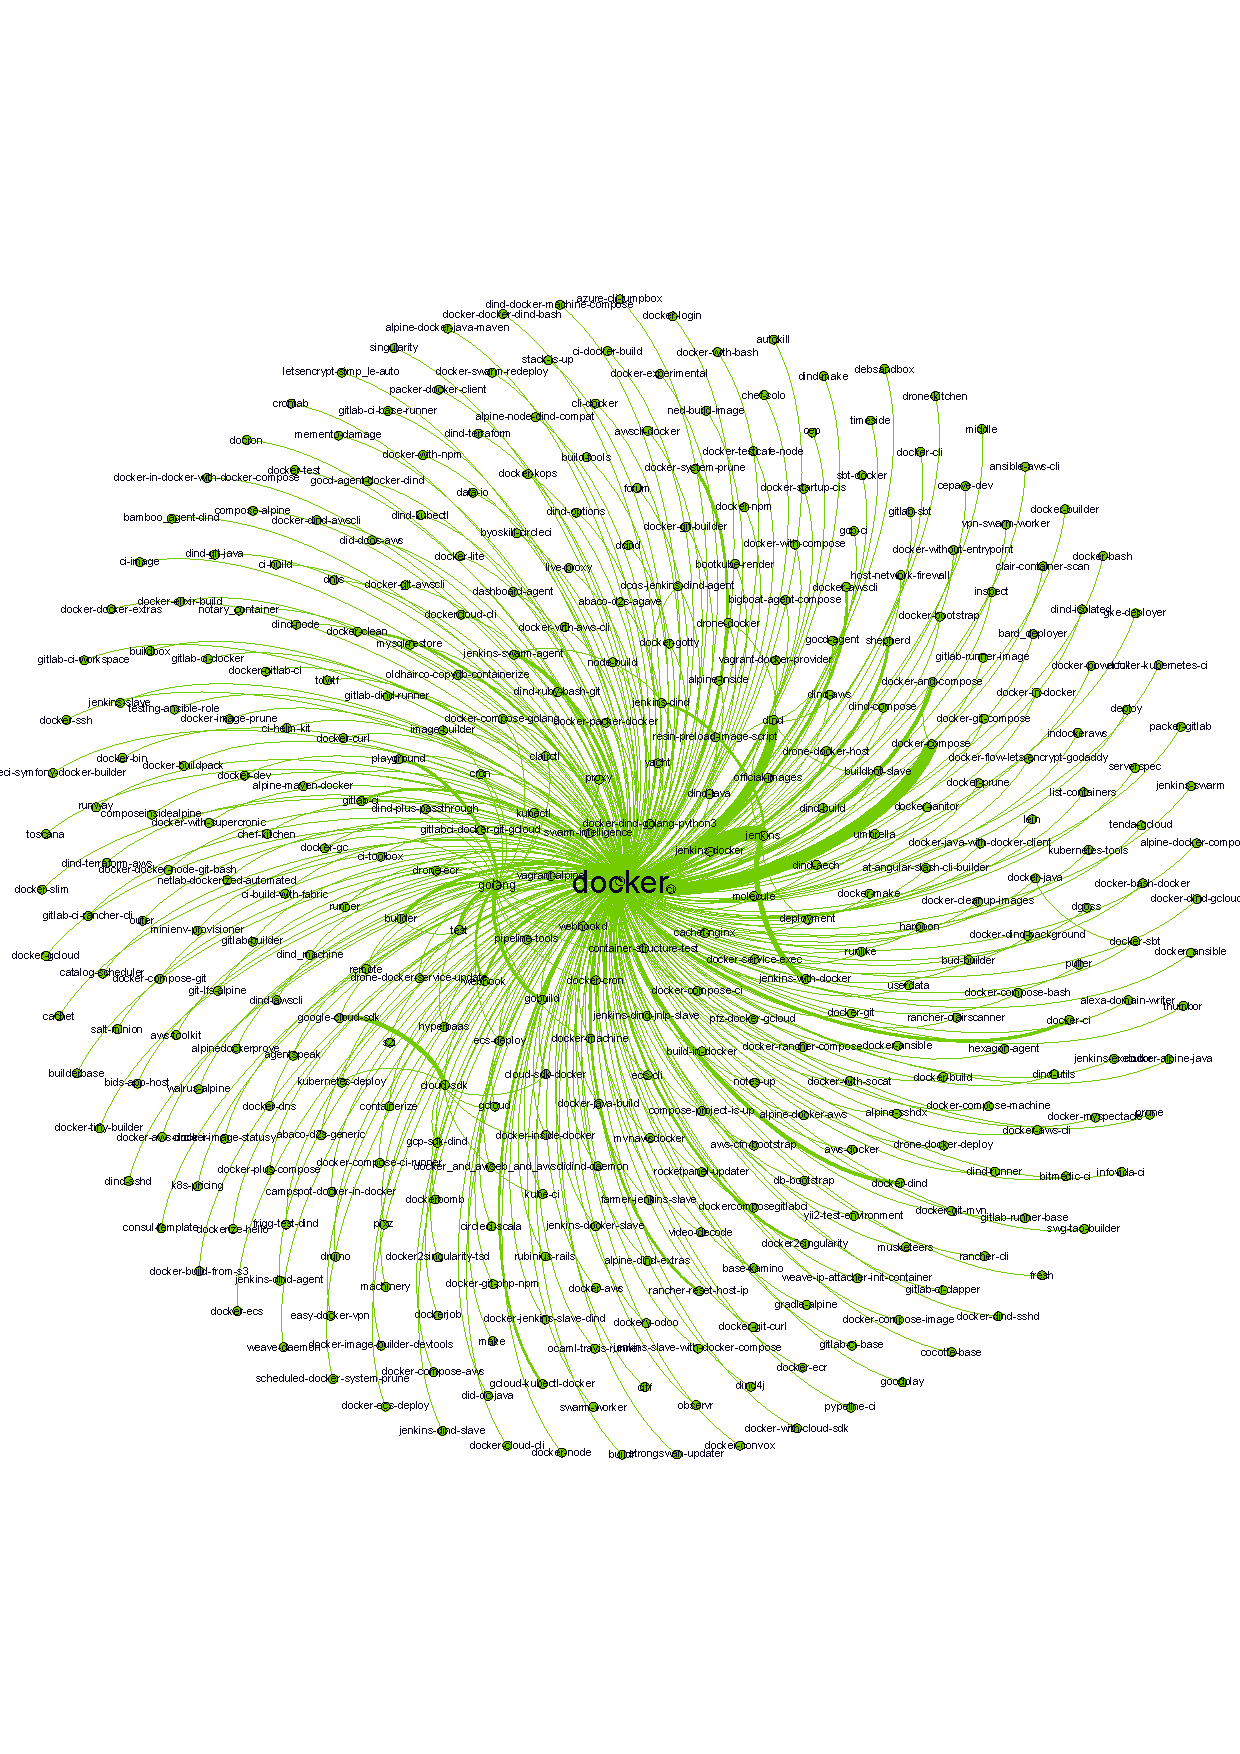
\includegraphics[width=1\columnwidth]{picture/image_network_docker1.pdf}\vspace{-0.3cm}
\caption{An example of subnetwork: docker.}
\label{fig:docker}
\end{figure}

% Table generated by Excel2LaTeX from sheet 'Sheet2'
\begin{table}[htbp]
  \centering
	\small
	\renewcommand\tabcolsep{2pt}
  \caption{Top-20 subnetworks ranked by interconnectedness.}\vspace{-0.3cm}
    \begin{tabular}{llrrrc}
   \toprule
    Subnetwork & Type  & \multicolumn{1}{l}{\#Nodes} & \multicolumn{1}{l}{\#Edges} & \multicolumn{1}{l}{$\sum$weights} & \multicolumn{1}{l}{Interconnectedness} \\
\midrule
    buildpack-deps & Other & 450   & 852   & 2,191  & 4.869  \\
    basecontainer & Other & 1,557  & 2,642  & 5,950  & 3.821  \\
    base  & Other & 952   & 1,720  & 3,295  & 3.461  \\
    apache & TS   & 71    & 93    & 245   & 3.451  \\
    centos7 & OS    & 68    & 93    & 230   & 3.382  \\
    scratch & Other & 681   & 1,102  & 2,214  & 3.251  \\
    alpine-glibc & OS    & 165   & 240   & 508   & 3.079  \\
    alpine-java & LR    & 194   & 275   & 586   & 3.021  \\
    opensuse & OS    & 100   & 144   & 299   & 2.990  \\
    base-alpine & OS    & 70    & 88    & 198   & 2.829  \\
    ubuntu & OS    & 14,976  & 22,535  & 38,577  & 2.576  \\
    openjdk & LR    & 1,686  & 2,437  & 4,328  & 2.567  \\
    composer & TS   & 125   & 183   & 315   & 2.520  \\
    alpine & OS    & 8,303  & 12,222  & 20,395  & 2.456  \\
    cuda  & AF  & 278   & 346   & 668   & 2.403  \\
    debian & OS    & 6,532  & 9,571  & 15,671  & 2.399  \\
    openresty & TS   & 67    & 72    & 160   & 2.388  \\
    centos & OS    & 3,689  & 5,273  & 8,630  & 2.339  \\
    alpine-oraclejdk8 & LR    & 126   & 150   & 261   & 2.071  \\
    fedora & OS    & 746   & 962   & 1,533  & 2.055  \\
\bottomrule
    \end{tabular}%
  \label{tab:subnetworks}%
\end{table}%



\noindent\textbf{Results}. 
Figure~\ref{fig:docker} gives the subnetwork we constructed for the container \emph{docker}\footnote{https://hub.docker.com/\_/docker}. 
Obviously, core container \emph{docker} occupies the center of this subnetwork. We also find that some parts of satellite containers also connected with each other. 
Further, for the Top-100 dominant containers found in RQ3, 
we construct their subnetworks and classify them into 5 categories. 
In total, 42 out of 100 subnetworks belong to the \emph{TS} category, 
21 subnetworks belong to the \emph{OS} category, 18 subnetworks belong to the \emph{LR} category, and 11 subnetworks belong to the \emph{AF} category. 
Thus, tools and services are the most common type in the container subnetworks, followed by the operating systems, language runtime, and application framework. 
%Interestingly,  we find these \emph{subnetwork:core containers} are mainly used for supporting software or container development. Detailed, of the TOP-100 \emph{subnetwork:core containers}, there are 42 Tools/Services, 21 OS, 18 Language runtime, and 11 Application I/F.  All of them provide infrastructure, platforms, or tools in their own way.   

\begin{figure*}[!t]
  \centerline{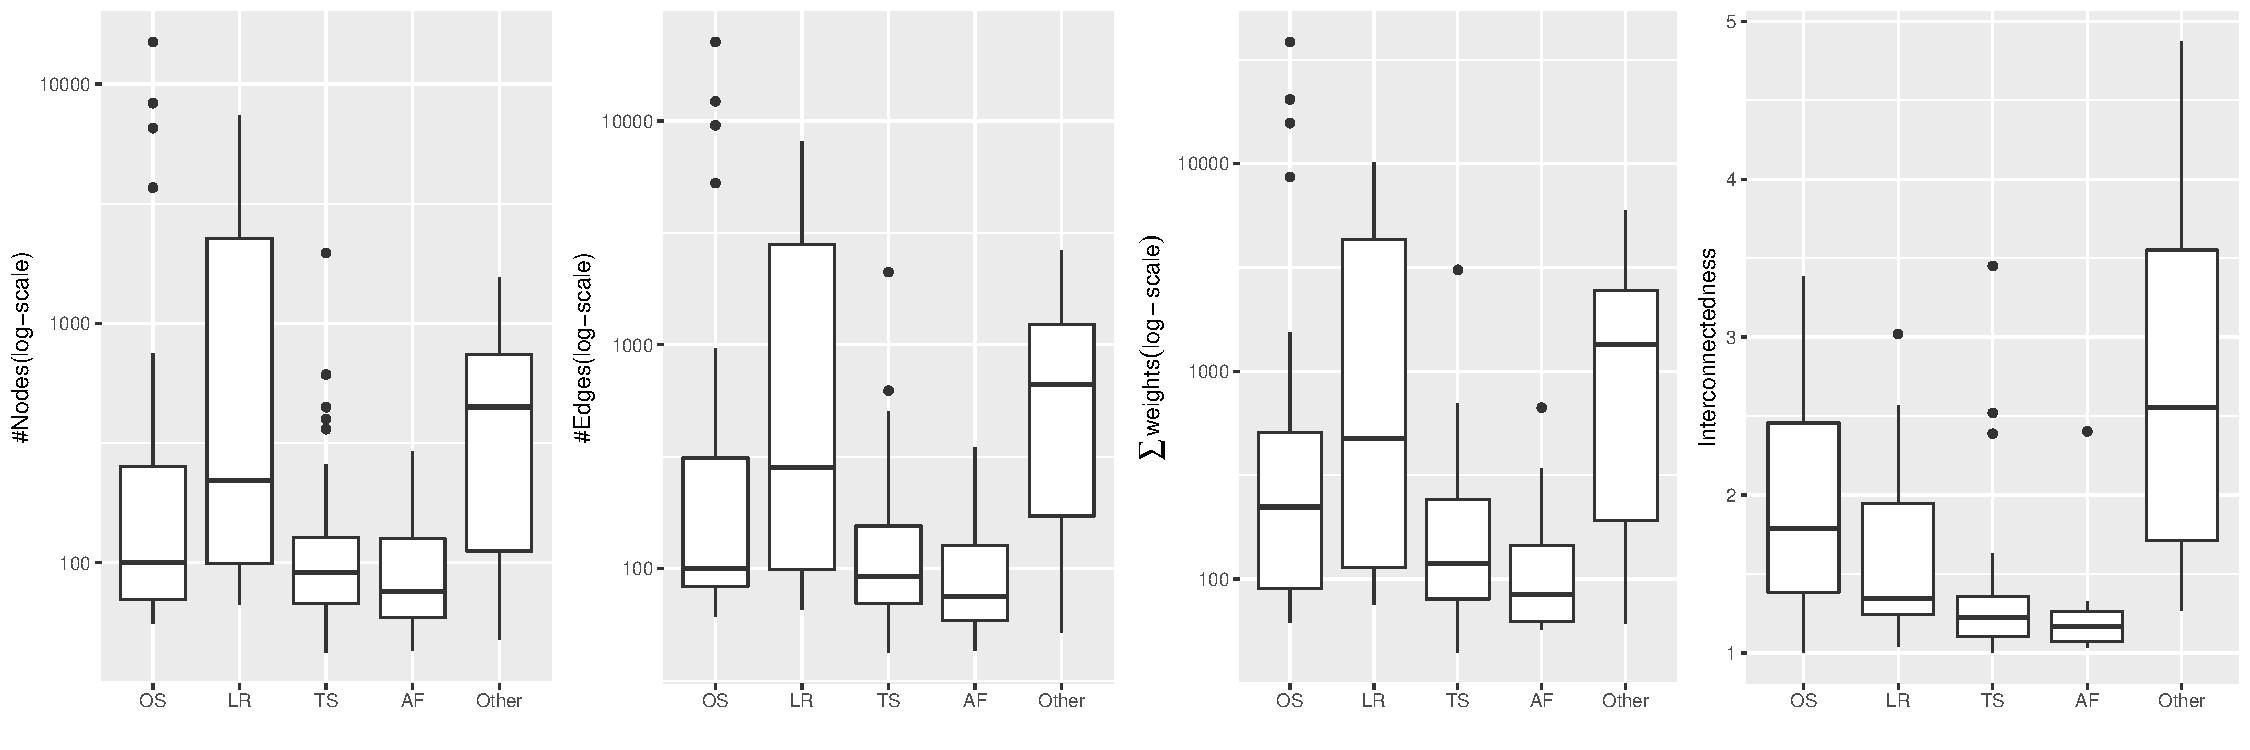
\includegraphics[width=1\textwidth]{picture/sub_coreimages_netstructre.pdf}}\vspace{-0.3cm}
  \caption{Comparison results of network metrics between subnetworks.}
  \label{fig:diversity}
  \end{figure*}

Table~\ref{tab:subnetworks} presents the detailed information of the Top-20 subnetworks ranked by the interconnectedness values.  
We find that container \emph{buildpack-deps} has the most interconnected network structure. \emph{buildpack-deps}\footnote{https://hub.docker.com/\_/buildpack-deps} is a collection of common build dependencies used for installing various modules, e.g., gems. 
Interestingly, we find that the subnetworks of \emph{base} and \emph{basecontainer} also have high interconnectedness. But they don't belong to a clear container application category. In the docker project \emph{headspinio/containerbase}\footnote{https://hub.docker.com/r/headspinio/containerbase}, the container was used to pre-install the apt package, while in the docker project  \emph{carrickpark/containerbase}\footnote{https://hub.docker.com/r/carrickpark/containerbase}, the container defines the base image of the \emph{carrickpark} application. In addition, in some dockerfiles, we 
find that the developer did not directly define the base image, but defined it by assigning a value to the ``\emph{base}'' variable. 
In general, the network structure and internal connectivity vary between subnetworks. Some small subnetworks (e.g., \emph{apache}) have relatively higher interconnectedness, while some big subnetworks (e.g., \emph{centos}) have relatively lower interconnectedness.


%Detailed metic information, in addition, can be seen in Table 2 ranked by \emph{LinksNumber/NodesNumber}. Subnetwork:buildpack-deps, providing containers building instruction set, has the most interconnected network structure, but its scale is average. Subnetwork:ubuntu, the biggest in all subnetworks, has a high value of interconnection.



\begin{mybox}
\emph{Answer to RQ4}: 
Tools and services are the most common type in the container subnetworks, followed by the operating systems, language runtime, and application framework. 
However, the network structure and internal connectivity of different subnetworks are diverse. 
%These \emph{subnetwork:core containers} are mainly used for supporting software or container development.
\end{mybox}






\subsection{RQ5: What is the difference between subnetworks?}\label{AA}
Next, we aim to investigate whether and to what extent do subnetworks differ from each other.

%\noindent\textbf{Motivation. } RQ2-1 has identified several detailed subnetworks and gave interpretable metrics to evaluate properties of subnetworks. To future understand properties presented by different subnetworks,  carrying out specific empirical research is essential. Thus, this RQ aims at investigating how and to what extend do subnetworks perform diversity in scale, interconnectedness between subnetworks across usage type to give deep insights into the properties of subnetworks. 


%Investigating the most tightly subnetworks in details is conducive to further obtain common feature and understand the reason for being tight subnetworks. 

% In addition, subnetworks constructed by different type influencial containers may undertake different functional aids in promoting docker containers universal and mantainced. Guide by the rule, we divide the influencial containers into several types including Operating System, Program language, Application service, Application framework etc as the TABLE 2 clearly shows. 


%However, differences scale and compactness of subnetworks may present a varirty of features, therefore it is important to investigate how and to what extend subnetworks performance diversity.

\noindent\textbf{Approach}. 
For the network metrics (i.e., \#nodes, \#edges, $\sum$weights, and interconnectedness), we use statistical methods to compare the differences between subnetworks. 
We mainly use Wilcoxon test~\cite{gehan1965generalized}, which is a non-parametric test, to compare the difference between two distributions.  We also compute Cliff's delta~\cite{macbeth2011cliff}, to measure the effect size that quantifies the difference between two distributions. 
Where the magnitude is assessed using the thresholds, i.e.,
$|\delta|$$<$0.147 ``negligible'', $|\delta|$$<$0.33 ``small'', $|\delta|$$<$0.474 ``medium'', otherwise ``large''. 
%To compare the differences between multiple distributions ($>$2), we use the Kruskal-Wallis test~\cite{}, which is an extension of the Wilcoxon test and can be used to test the hypothesis that a number of unpaired samples originate from the same population. 

%To compare diversity of subnetwork type, we aggregate our dataset per type according to usage for developing software to obtain the scale and interconnectedness differencees across subnetworks type. For each type, we computed the \emph{NodesNumber}, \emph{EdgesNumber} and \emph{LinksNumber} of each subnetwork.  
%To access the reliability of the results, we apply Wilcoxon test and Cliff’s delta to do significance test on differences results. 





\smallskip
\noindent\textbf{Results}. 
%Figure 3 shows the comparison boxplots. We find that different typse of influencial containers network may have different network structure. E.g.,Operating system subnetwork may have larger diameter and average shortest length. This may result from Operating system's larger subnetwork scale. Because of the build-form of the subnetwork always character as the star pattern(large amount of docker containers always central with one or minority docker containers)  
Figure~\ref{fig:diversity} shows the comparison boxplots between different types of subnetworks. %including scale metic as Nodesnumber, Edgesnumber, Linksnumber and interconnectedness metic Linksnumber/Nodesnumber differences across subnetworks type.  
For the basic scale metrics, we find that 
%\noindent\textbf{Scale. }We find that 
different types of subnetworks may vary. 
The detailed hypothesis test results are shown in Table~\ref{tab:hypo}. 
Especially, the subnetworks of \emph{LR} have more nodes, more edges, and larger weights. Their network scales are significantly larger than the subnetworks of \emph{TS} and \emph{AF} ($p$-value$<$0.05; effect size is large). 
%hypothesis test showed as Table3. 
This is as expected, since \emph{LR} being essential basic conditions for realizing software functions will have a wider range of usage than \emph{AF} or \emph{TS} biased towards implementing a specific function or application in a specific field. E.g., container \emph{Redis} is used as a database and container \emph{Tomcat} is used as a web server. 
Interestingly, we find there are several outliers in the boxplots of \emph{OS} subnetworks. We manually check and find that
those 
%ranked the second among the four containers types but with several abnormal containers including ubuntu, alpine etc. The reason may be that these several 
abnormal containers are extremely popular even compared with other \emph{OS} containers, e.g., \emph{Ubuntu} and \emph{alpine}. 
However, the scale differences between \emph{OS} and \emph{LR} are not significant.
%Compared with the obvious clustering effect of OS selection, the differences between different LR are not so obvious, identifying that each LR has its own adaptive population.  Thus, maintenance of these extremely popular container is worth our attention. 

% Table generated by Excel2LaTeX from sheet 'Sheet1'
\begin{table}[!t]
  \centering
  \renewcommand\tabcolsep{2pt}
  \small
  \caption{Hypothesis test results between different groups.}\vspace{-0.3cm}
    \begin{tabular}{lccccccccc}
\toprule
          & \multicolumn{3}{c}{\#Nodes} & \multicolumn{3}{c}{\#Edges} & \multicolumn{3}{c}{$\sum$Weights} \\
    Group & $p$-value & $|\delta|$ & effect & $p$-value & $|\delta|$ & effect & $p$-value & $|\delta|$ & effect\\
\midrule
    LR-AF & 0.011  & 0.566  & *** & 0.008  & 0.586  & *** & 0.004  & 0.626  & *** \\
    LR-TS & 0.003  & 0.488  & *** & 0.002  & 0.504  & *** & 0.002  & 0.509  & *** \\
    LR-OS & 0.143  & 0.278  & * & 0.291  & 0.201  & * & 0.364  & 0.175  & * \\
    AF-TS & 0.511  & 0.132  & - & 0.490  & 0.139  & - & 0.334  & 0.193  & * \\
    AF-OS & 0.226  & 0.268  & * & 0.088 & 0.377  & ** & 0.340  & 0.463  & ** \\
    TS-OS & 0.374  & 0.139  & - & 0.120  & 0.243  & * & 0.067  & 0.287  & * \\
\bottomrule
 \multicolumn{10}{l}{`***' large, `**' medium, `*' small, `-' negligible}\\
    \end{tabular}\vspace{-0.3cm}
  \label{tab:hypo}%
\end{table}








%nodenumber PAF lr 0.0108  -0.5656566   large  PTS lr 0.0030  -0.4880952   large
%edgenumber PAF lr 0.00809890  -0.5858586 large  PTS lr 0.00217639  -0.5039683 large
%all_edgesnumber  PAF lr 0.004341380  -0.6262626 large  PTS lr 0.001951463   -0.5092593 large


%Actually, the scale of these sub network of core containers reflect the directly connected containers.
 



As for the interconnectedness, we find that \emph{OS} subnetworks have 
larger values than other types of subnetworks. Specifically, the difference between \emph{OS} and \emph{LR} is medium ($p$-value$<$0.05; Cliff's delta=0.36), the difference between \emph{OS} and \emph{AF} ($p$-value$<$0.05; Cliff's delta=0.55), \emph{OS} and \emph{TS} ($p$-value$<$0.05; Cliff's delta=0.51), are large. 
%rate  AF OS 0.01075928  -0.5497835 (large)     TS OS  0.00109008   -0.5090703 (large)     TS  LR 0.02767026    -0.3624339 (medium)   
%From the the rightest comparison boxplots showed in Figure 5, interconnectedness of OS subnetworks values higher than  interconnectedness of AF subnetworks (Wilcoxon test, p=0.0108; Cliff’s delta, p= -0.550, large) and TS subnetworks (Wilcoxon test, p=0.001; Cliff’s delta, p = -0.509, large). 
This indicates that containers in the \emph{OS} subnetworks have more connectivity. \emph{OS} only provides a basic operating environment, applications and tools may need to depend on each other and be combined to achieve complete container functions.    





\begin{mybox}
\emph{Answer to RQ5}: 
There exist some differences in the network metrics between different types of subnetworks. Especially, \emph{LR} subnetworks tend to have a large scale, while \emph{OS} subnetworks are associated with higher interconnectedness.
%as well as OS subnetworks, have the most compact structure while AF subnetworks value small both in scale and compactness. 
\end{mybox}









\subsection{RQ6: How connected are the subnetworks?}
%Base on the above analyse, it is the several From instructions that resulting the interactive relationships between docker containers. To further explore the stronger relationship between subnetworks and the several FROM instructions distribution and reasons between docker containers, we list the TOP-20 strongest realtionships between docker containers as TABLE2 shows.

Finally, we seek to explore the relationship between subnetworks. 
%\noindent\textbf{Motivation. }
%Diversity of subnetworks, focusing on differences in scale and compactness of different subnetworks types has been investigated in depth in RQ2-2. Since core containers are proved not to be isolated, therefore we also have reason to believe the connection relationship between subnetworks. Thus, deep insights into the connection relationship between subnetworks and effect of usage type of subnetworks on the connection relationship need further research. Significantly, identify connection relationshps between subnetworks can be used to recommend associated containers.


%By answering these  questions, we can perceive the overview of relationships between different type of subnetworks. The stronger relationships pairs captured may be a singal of coorporate realitinshp for software development. We can use it to capture the relationships feature for containers recommendation according to their similar feature or coorporate feature.


%Core containers may directed to other containers belonging to other subnetwork, One container, interestingly, may direct to different containers belonging to different subnetworks that reflect subnetworks are not isolated. Further, deep insights into the more stronger relationships is           
%necessary. In other words, 


\noindent\textbf{Approach}. 
%\emph{\textbf{1) choose metic. }}
To measure the inter-connection between two subnetworks, we define the \emph{connection-strength}, i.e., the sum of the edge weights of the intersecting nodes of the two subnetworks. For example, the \emph{connection-strength} between subnetwork A and subnetwork B is 10 (1+3+2+4), as shown in Figure~\ref{fig:conndefine}.
%It is calculated as follow: 
\begin{equation}
Connection-strength = \sum weight_{intersection}\label{eq}
\end{equation}


\begin{figure}[htbp]
\centering
  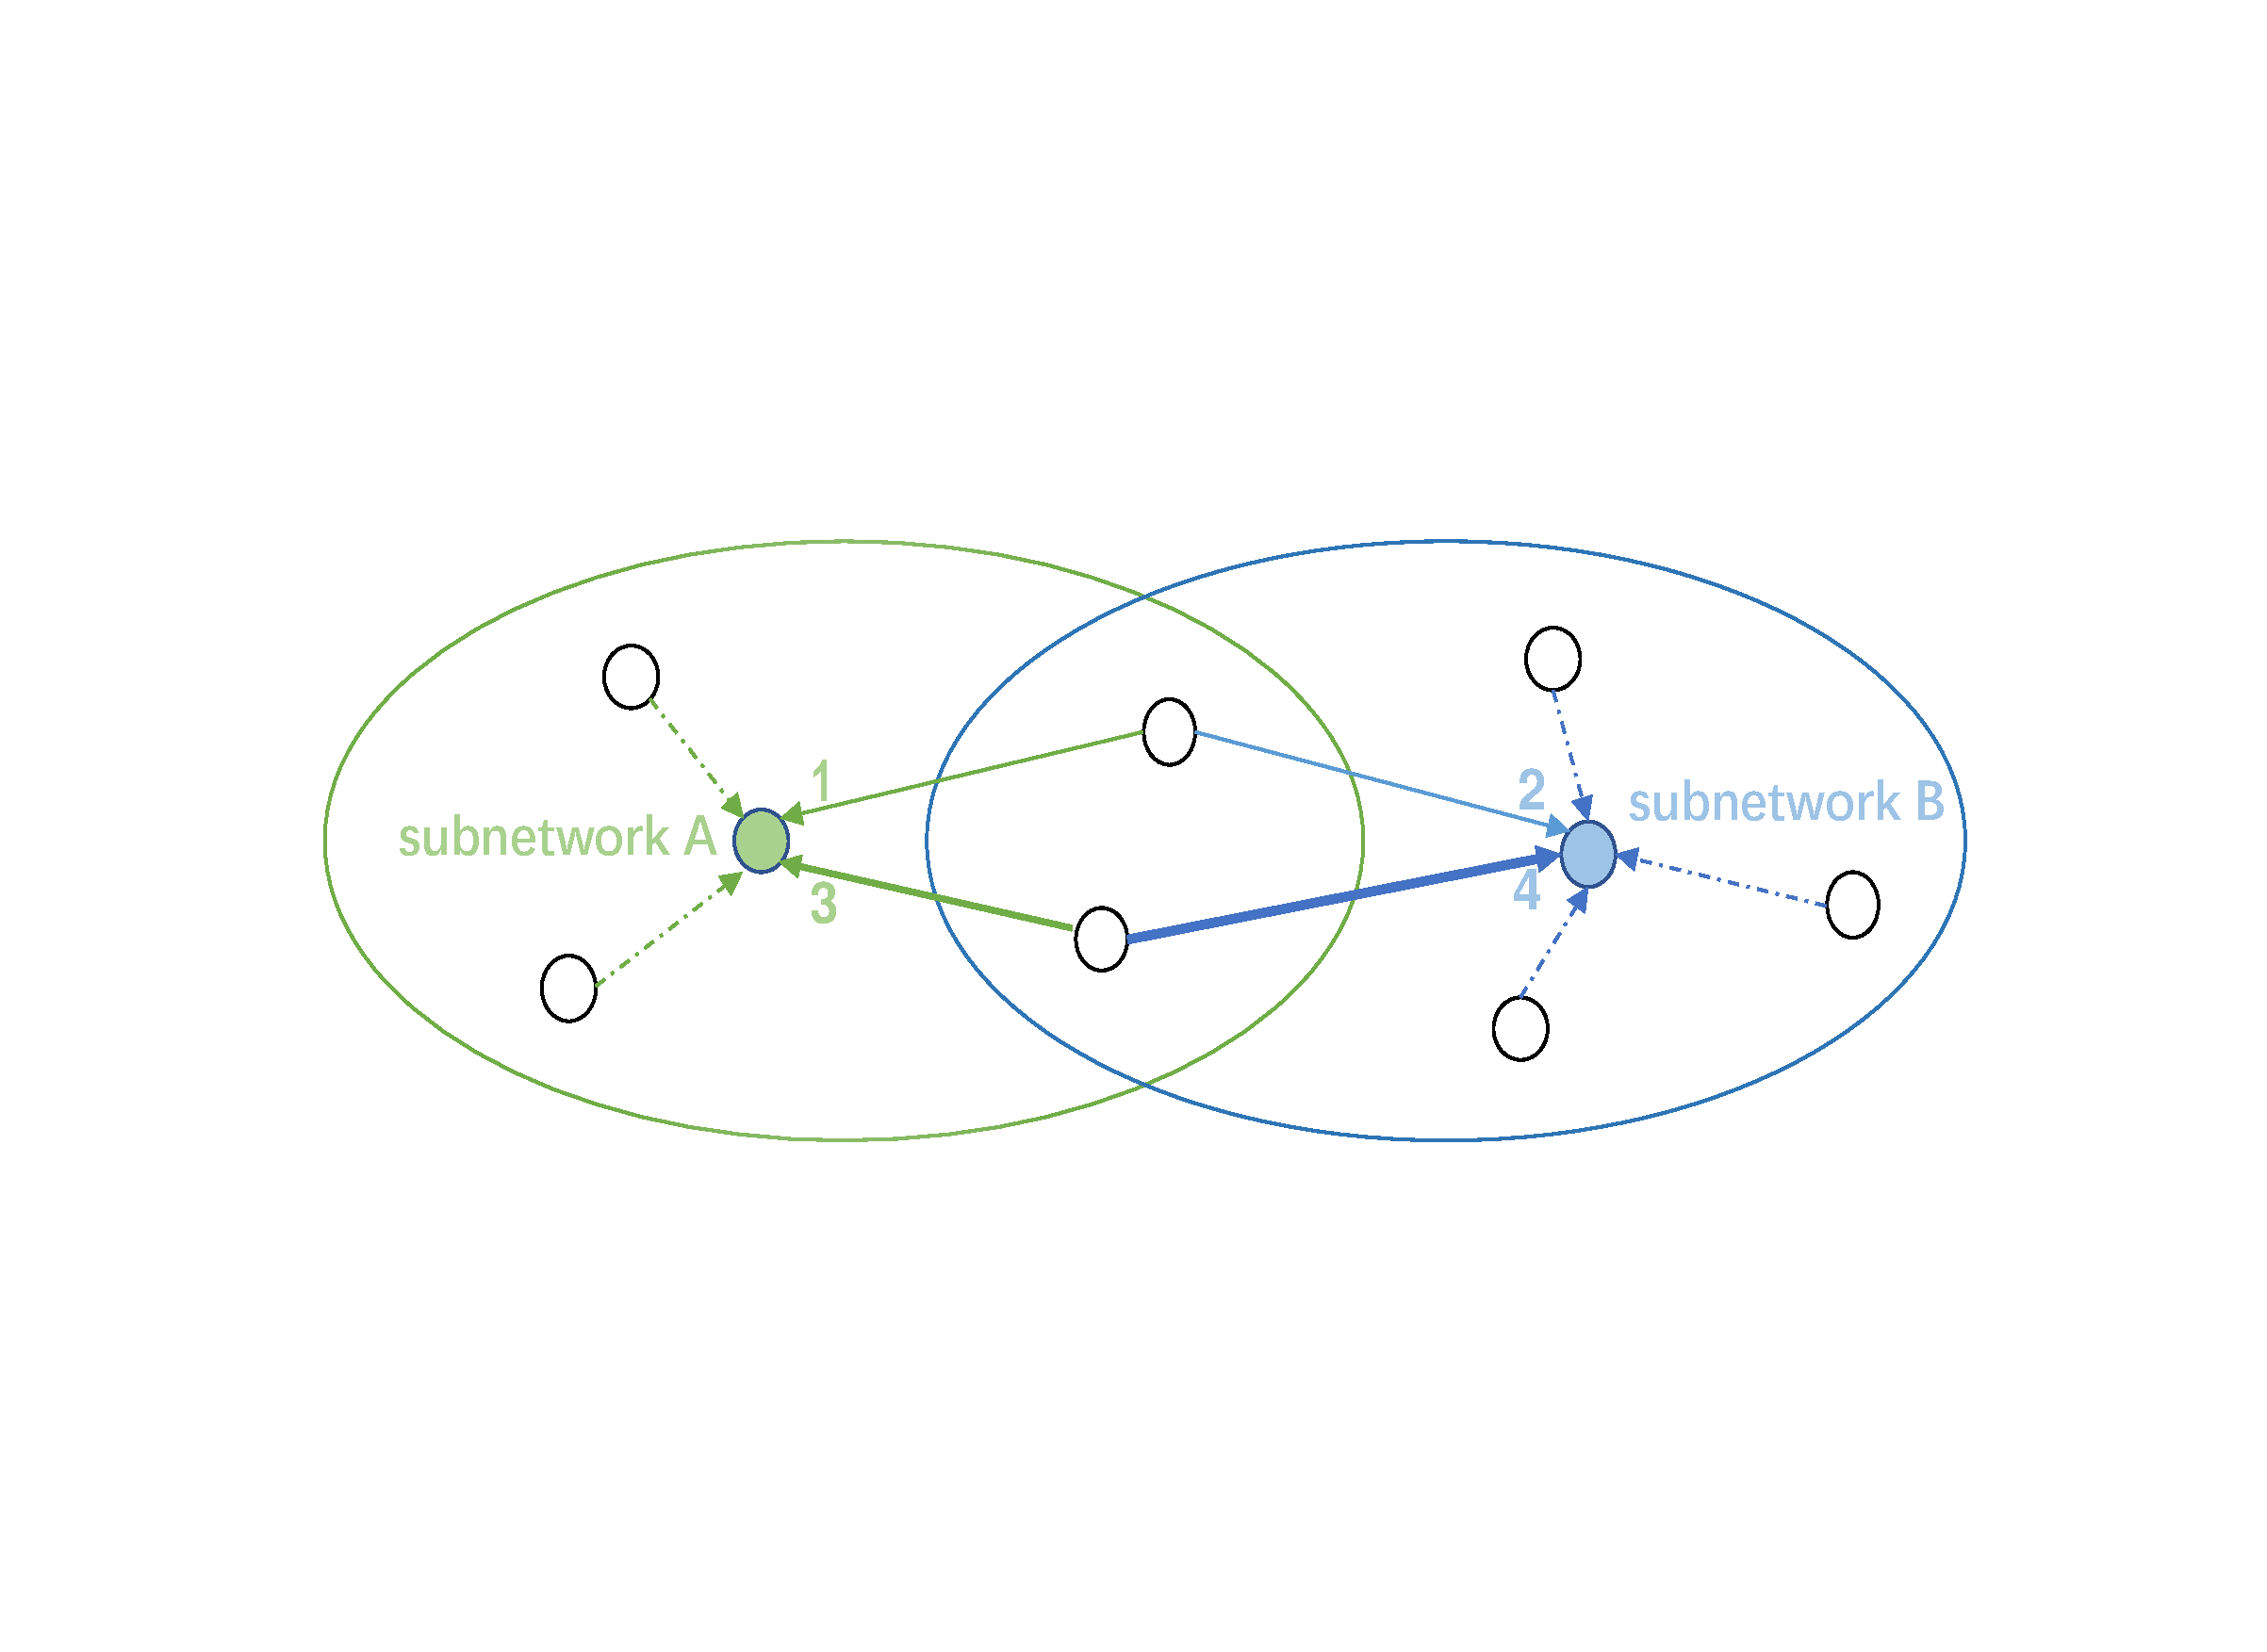
\includegraphics[width=0.9\columnwidth]{picture/connection5.pdf}
\caption{Example of computing the connection-strength.}
\label{fig:conndefine}
\end{figure}



%Noticeably, the intersection nodes between subnetworks are direct metic to represent \emph{Connection strength}, however, ignoring the dependence frequency of different nodes. The edges attached with labeltimes between intersection containers and core containers seems the best solution to character \emph{Connection strength} between subnetworks. 



%Intuitively, the cross spots belonging to two subnetworks meanwhile represent linking relationships between subnetworks. Further, we defined the \emph{linking strength} between subnetworks as the the edges times between crossspots and core containers multipy frequency labels, symbolized as \emph{linking strength} = \emph{edge} * \emph{timeslabel}. 

%\emph{\textbf{2) computation and classify. }} 
We compute the \emph{connection-strength} between each two of the 100 subnetworks. %and identify strong relationships between subnetworks. Next, 
Then, we mark each connected subnetwork group using their 
categories as defined in RQ4. E.g., \emph{OS} subnetwork and \emph{LR} subnetwork should be marked as \emph{OS-LR}. 
Note that we mark the subnetwork group as \emph{Other} if one of the subnetworks belong to the \emph{Other} category. %we classify subnetwork pairs based on classification results of single subnetwork in RQ1-1. Specifically, 
%we combined the type of each subnetwork as the type of subnetwork pairs, eg., type of subnetwork pair containing subnetwork:OS and subnetwork:LR are defined as OS-LR. Specially, we say type of subnetworks pairs as Other if it contains a subnetwork whose type is classified as Other. 
%\emph{\textbf{3) hypothesis test. }} 
To compare the differences of \emph{connection-strength} between different types of subnetwork groups, we use the Kruskal-Wallis test~\cite{mckight2010kruskal}, which is an extension of the Wilcoxon test and can be used to test the hypothesis that a number of unpaired samples originate from the same population. 
%we investigate different types of subnetwork pairs differing in \emph{connection strength}. To describe and further verify differential results, we create boxplots and do Kruskal-Wallis tests on differential results.

\smallskip
\noindent\textbf{Results}. 
Based on the 100 subnetworks, we compute the \emph{connection-strength} %Interconnection of 100 subnetworks centralized with top-100 core containers result in 
of 4,950 subnetwork groups, in which 11 subnetworks groups belong to the \emph{Other}. 
When we look at the Top-100 subnetwork groups ranked by the \emph{connection-strength}, we find that 30\% groups belong to the \emph{OS-LR}, 
28\% groups belong to the \emph{OS-OS}, 14\% groups belong to the \emph{LR-LR} or \emph{OS-TS}, and 3\% groups belong to the \emph{LR-TS} or \emph{OS-AF}.  
Specifically, Table~\ref{tab:rel} shows the list of Top-20 subnetwork groups ranked by the \emph{connection-strength}. We find that the \emph{OS-OS} group ranks very high. 
Next, we compare the differences of \emph{connection-strength} between different types of subnetwork groups, as shown in Figure~\ref{fig:connection distribution}. 
%Regardless of
%Due to their fuzzy features, we filtered subnetwork pairs whose type is classified as Other. 
%We then analyzed and a draw boxplot about \emph{connection strength} on the remainder 10 kinds of subnetwork pairs showed in Figure~\ref{fig:connection distribution}. 
%We can get an obvious rule of connection relationship between subnetworks: OS-OS OS-LR LR-LR OS-AF OS-TS has stronger \emph{connection strength} indicating closer tie while relationship between TS-AF TS-TS AF AF is relatively more looser (Kruskal-Wallis p<0.001).
The distribution of \emph{connection-strength} per type of subnetwork group is significantly different (Kruskal-Wallis test; p$<$0.001); Thus, we find that the types of subnetwork groups may have impact on the \emph{connection-strength}. 
%\vspace{-0.3cm}
%Figure 6 gives vivid example of subnetwork:maven and subnetwork:tomcat. Maven and tomcat occupies the central position in each sub network, and both of them emerg technical dependencies with some common containers. 


%Showed as Table 4, top-20 most tightly connected subnetwork pairs can be obviously observed attached with \emph{connection strength} and \emph{Type-Pairs} results. We also Statisticed the most noteworthy top-100 subnetwork pairs, among them OS-LR(count=30), OS-OS(count=28) are the most tightly connected subnetwork pairs, followed by LR-LR(count=7) and OS-TS(count=7). The rest are LR-TS(count=2), OS-AF(count=1) and Other(count=25). Especially, java and openjdk are actually the same container with different names.  

% Table generated by Excel2LaTeX from sheet 'corecontainers_network_crossspots'
\begin{table}[htbp]
  \centering
  \small
  \caption{Top-20 subnetwork groups.}\vspace{-0.3cm}
    \begin{tabular}{lllc}
	\toprule
    Subnetwork1 & Subnetwork2 & Group & \multicolumn{1}{l}{Connection strength} \\
	\midrule
    ubuntu & alpine & OS-OS & 7,487 \\
    ubuntu & debian & OS-OS & 7,391 \\
    alpine & debian & OS-OS & 5,665 \\
    ubuntu & centos & OS-OS & 4,194 \\
    golang & alpine & OS-LR & 2,833 \\
    ubuntu & basecontainer & Other & 2,772 \\
    ubuntu & base  & Other & 2,550 \\
    centos & alpine & OS-OS & 2,523 \\
    node  & ubuntu & OS-LR & 2,329 \\
    centos & debian & OS-OS & 2,329 \\
    python & ubuntu & OS-LR & 2,303 \\
    alpine & base  & Other & 2,095 \\
    ubuntu & java  & OS-LR & 1,925 \\
    alpine & basecontainer & Other & 1,905 \\
    php   & ubuntu & OS-LR & 1,881 \\
    basecontainer & debian & Other & 1,791 \\
    python & alpine & OS-LR & 1,775 \\
    base  & debian & Other & 1,751 \\
    java  & openjdk & LR-LR & 1,688 \\
    ubuntu & openjdk & OS-LR & 1,558 \\
	\bottomrule
    \end{tabular}%
  \label{tab:rel}%
\end{table}%



\begin{figure}[htbp]
\centerline{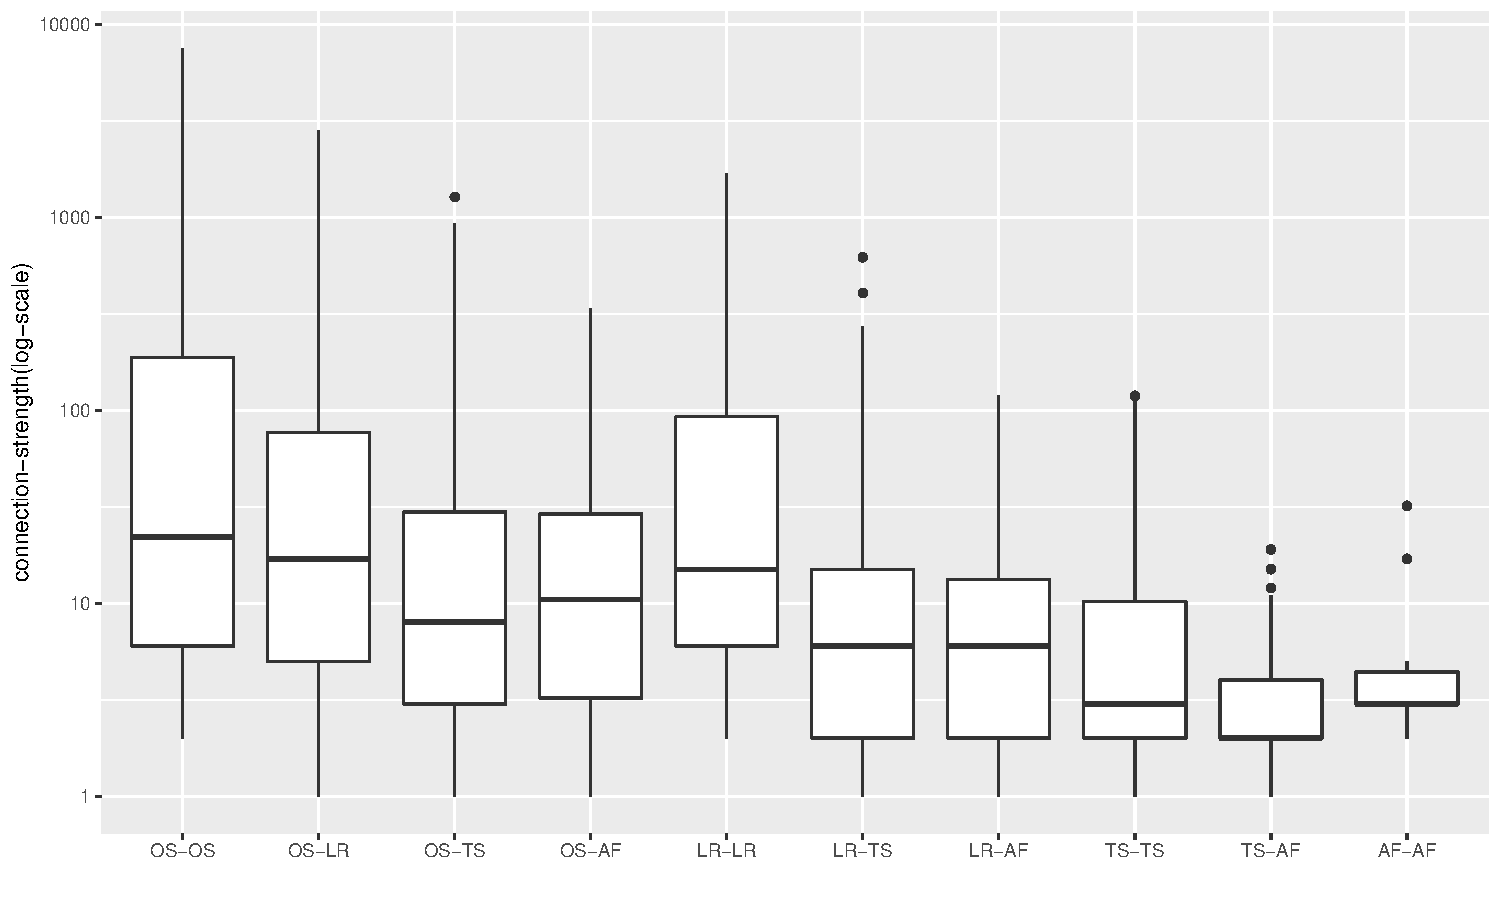
\includegraphics[width=0.48\textwidth]{picture//typepairs_linkstrength.pdf}}\vspace{-0.3cm}
\caption{Comparison of the \emph{connection-strength} between different subnetwork groups.}
\label{fig:connection distribution}
\end{figure}






\begin{figure}[htbp]
\centerline{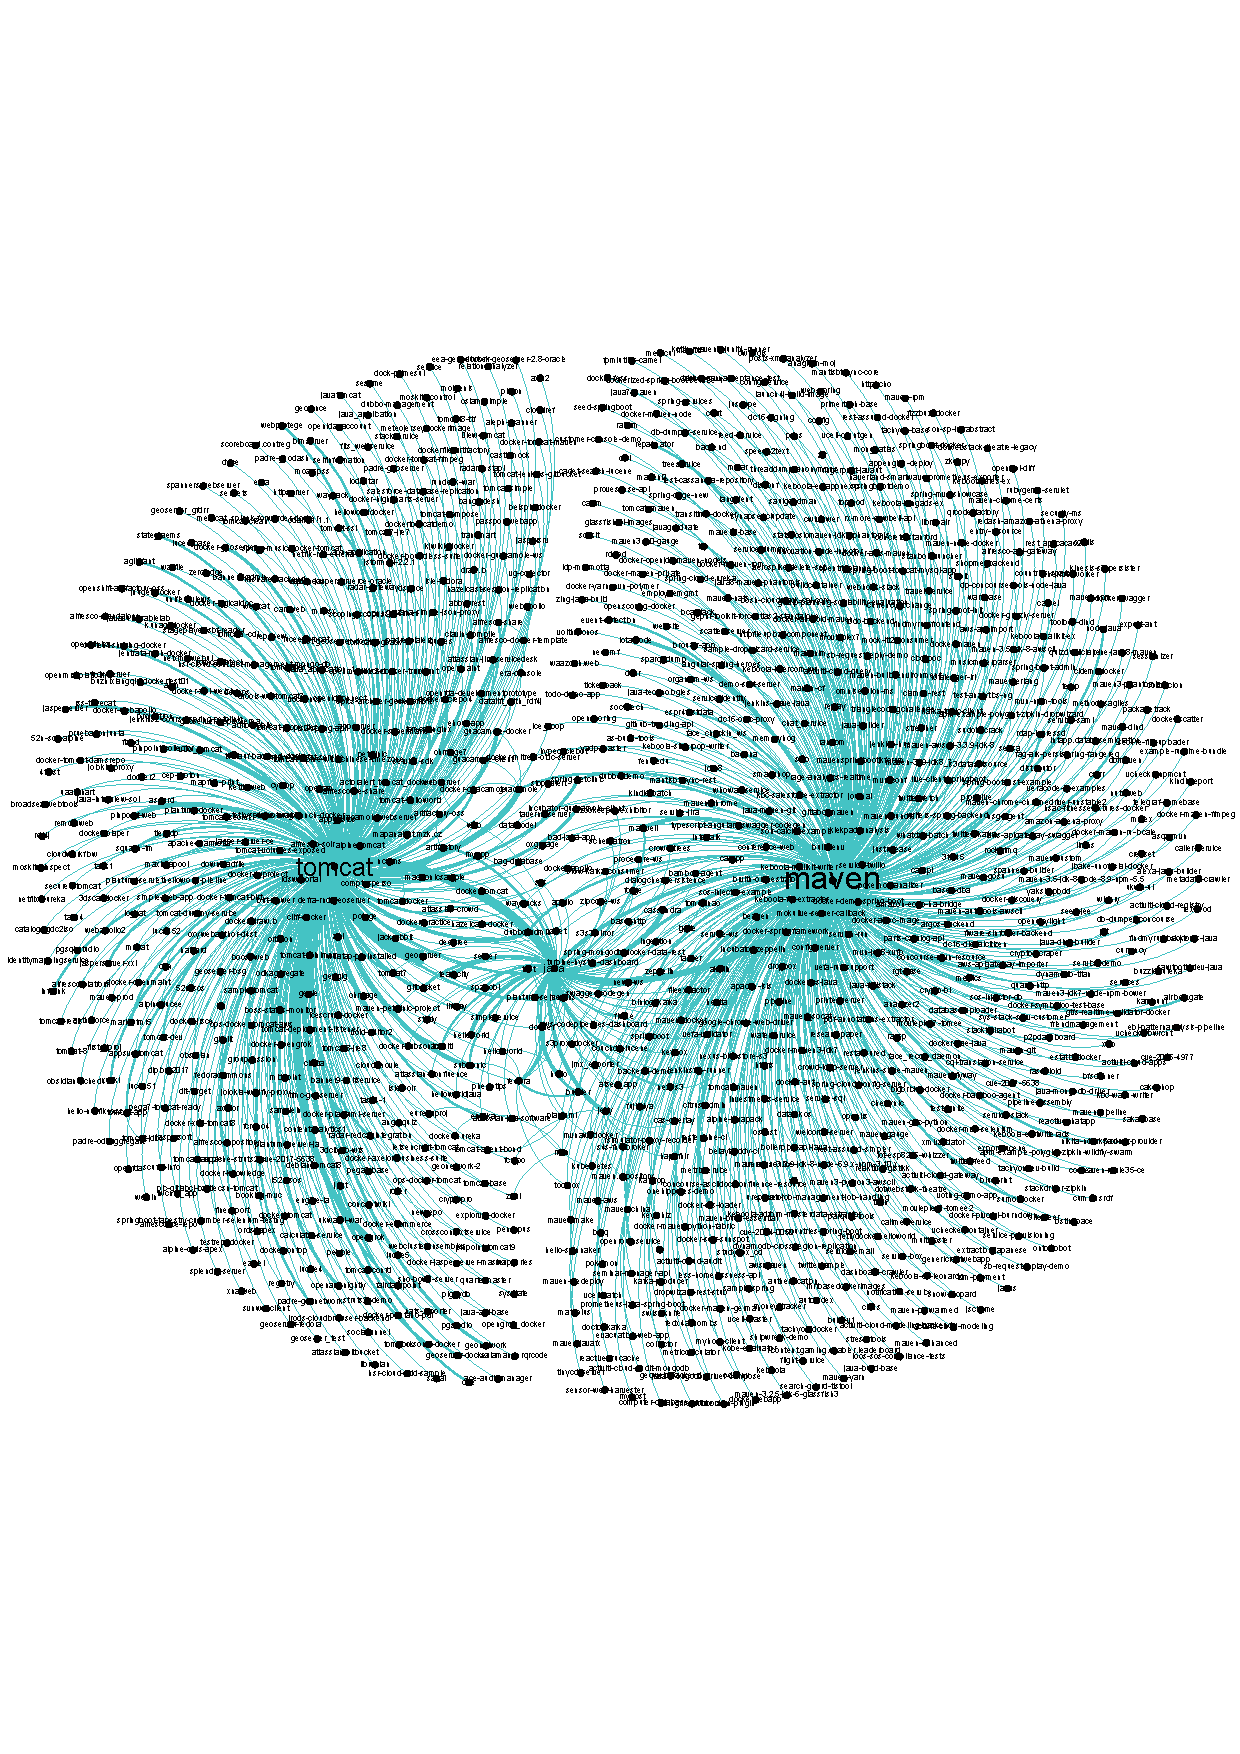
\includegraphics[width=0.48\textwidth,trim=10 130 10 130,clip]{picture//image_network_pairs_maven_tomcat22.pdf}}
\caption{The joint network of Tomcat and Maven.}
\label{fig:maven-tomcat}
\end{figure}


% this one can be removed
%\begin{figure}[htbp]
%centerline{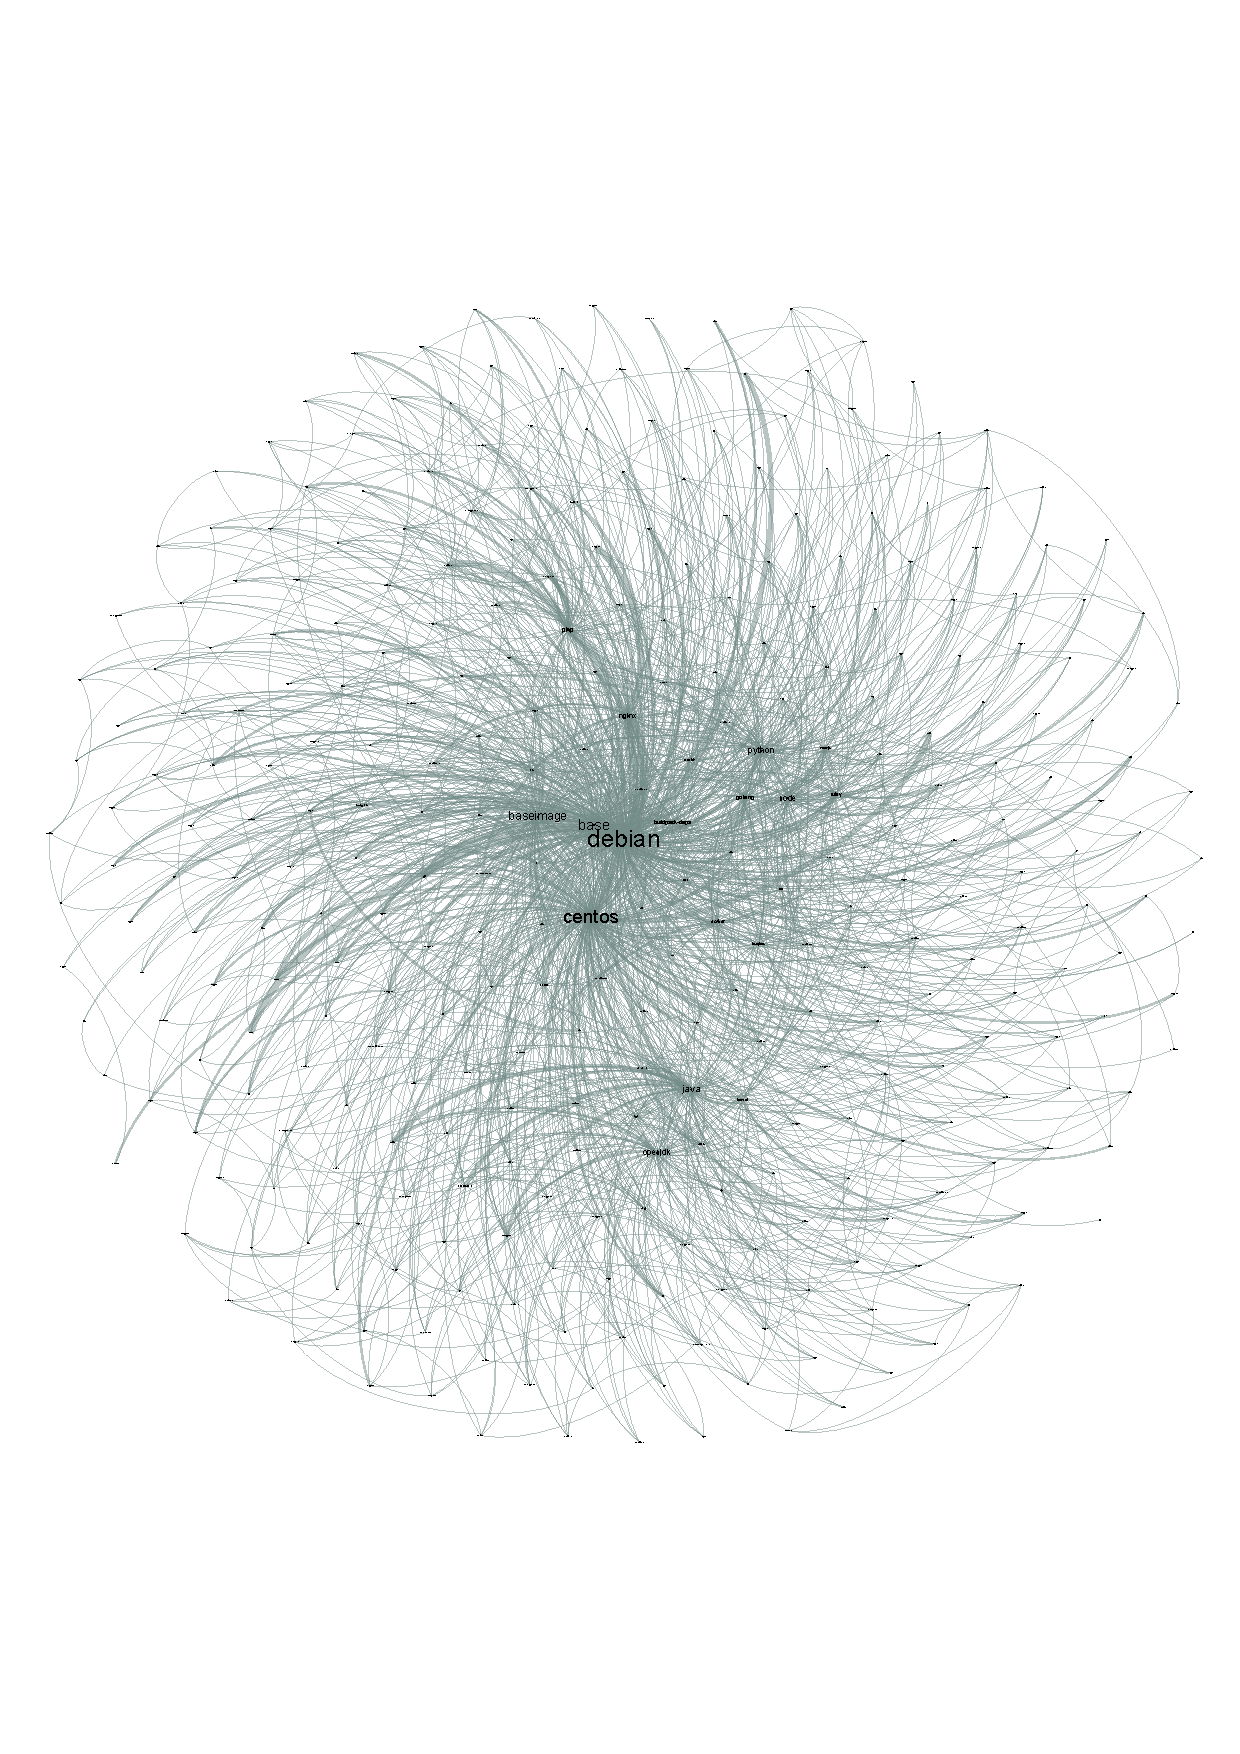
\includegraphics[width=0.35\textwidth,trim=10 130 10 %130,clip]{picture//image_network_pairs_centos_debain3.pdf}}
%\caption{The joint network of Centos and Debian.}
%%\label{fig:centos-debain}
%\end{figure}



\begin{figure}[htbp]
\centerline{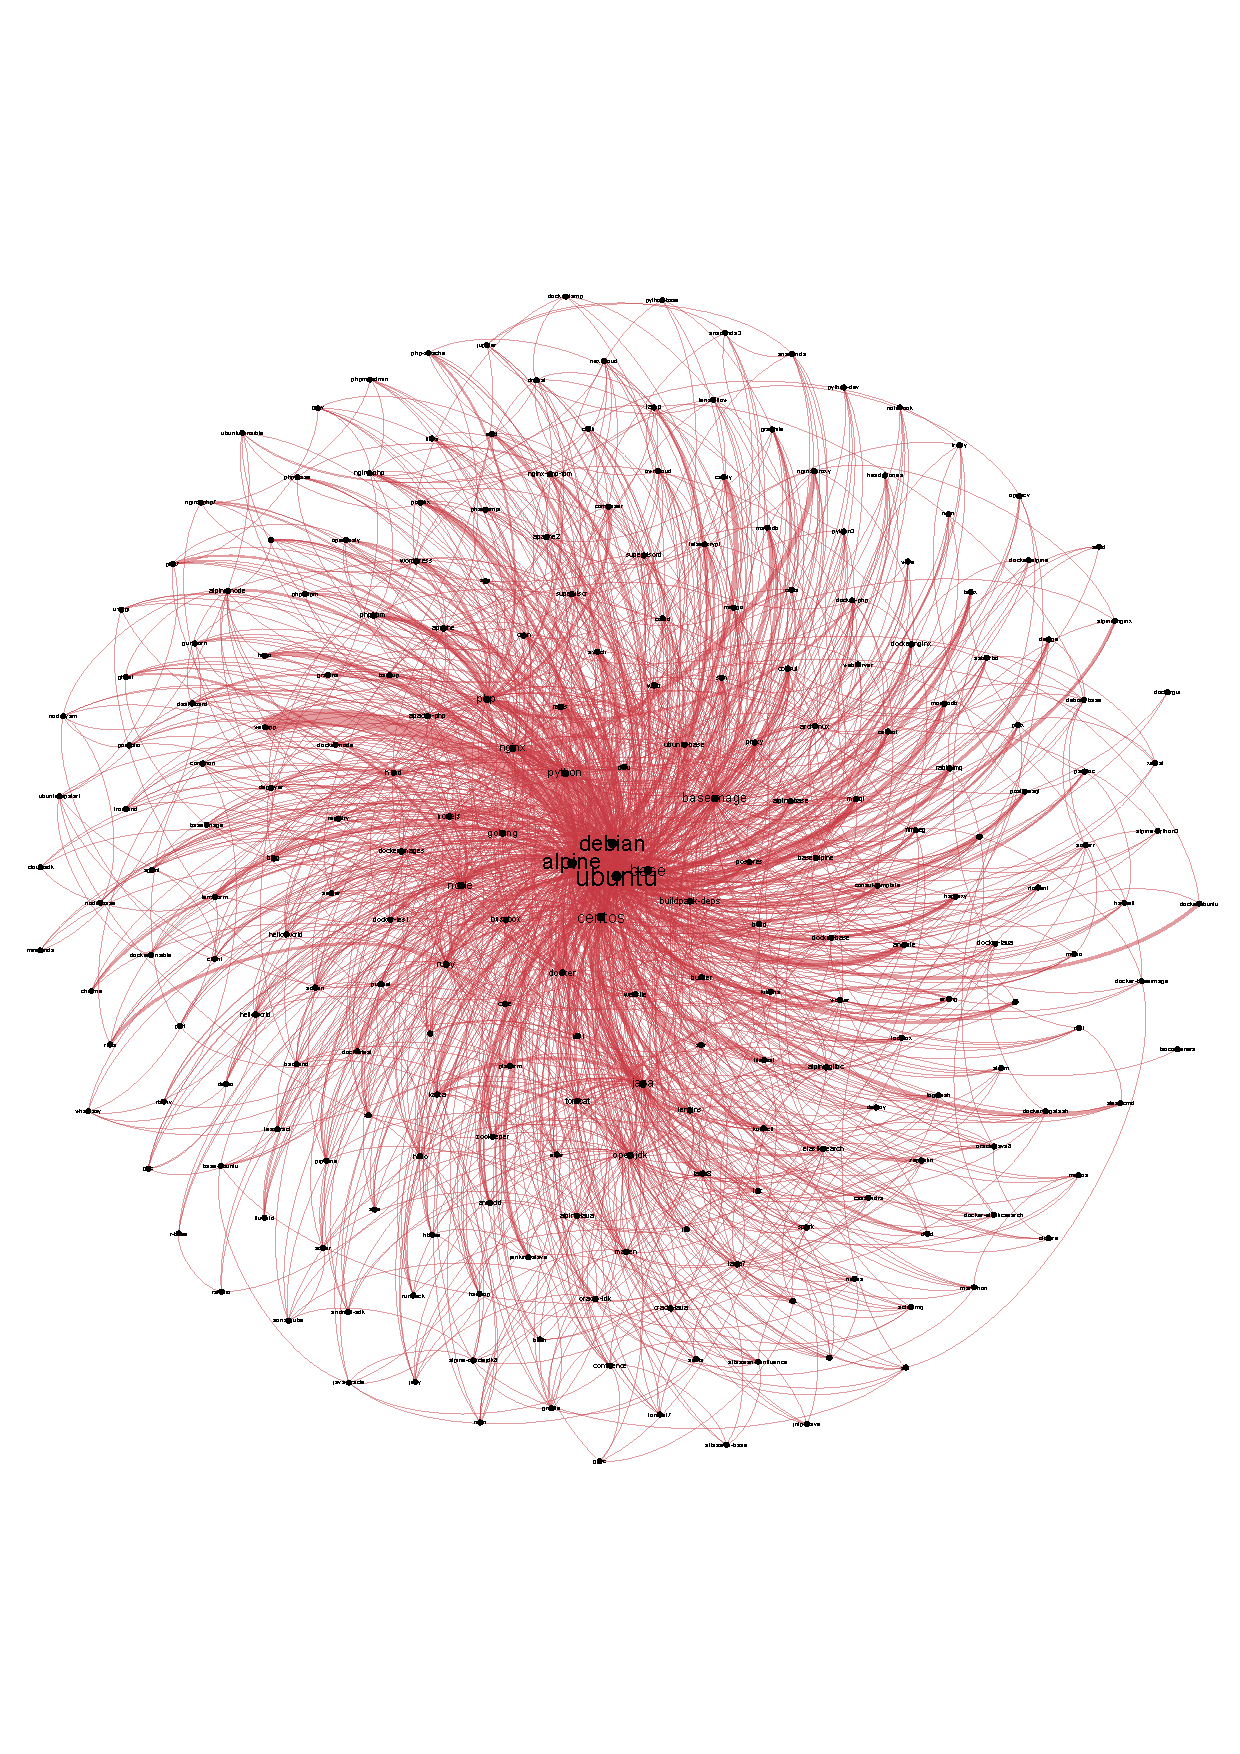
\includegraphics[width=0.45\textwidth,trim=10 130 10 130,clip]{picture//image_network_pairs_ubuntu_alpine2.pdf}}
\caption{The joint network of Ubuntu and Alpine.}
\label{fig:ubuntu_alpine}
\end{figure}


%\begin{figure}[htbp]
%\centerline{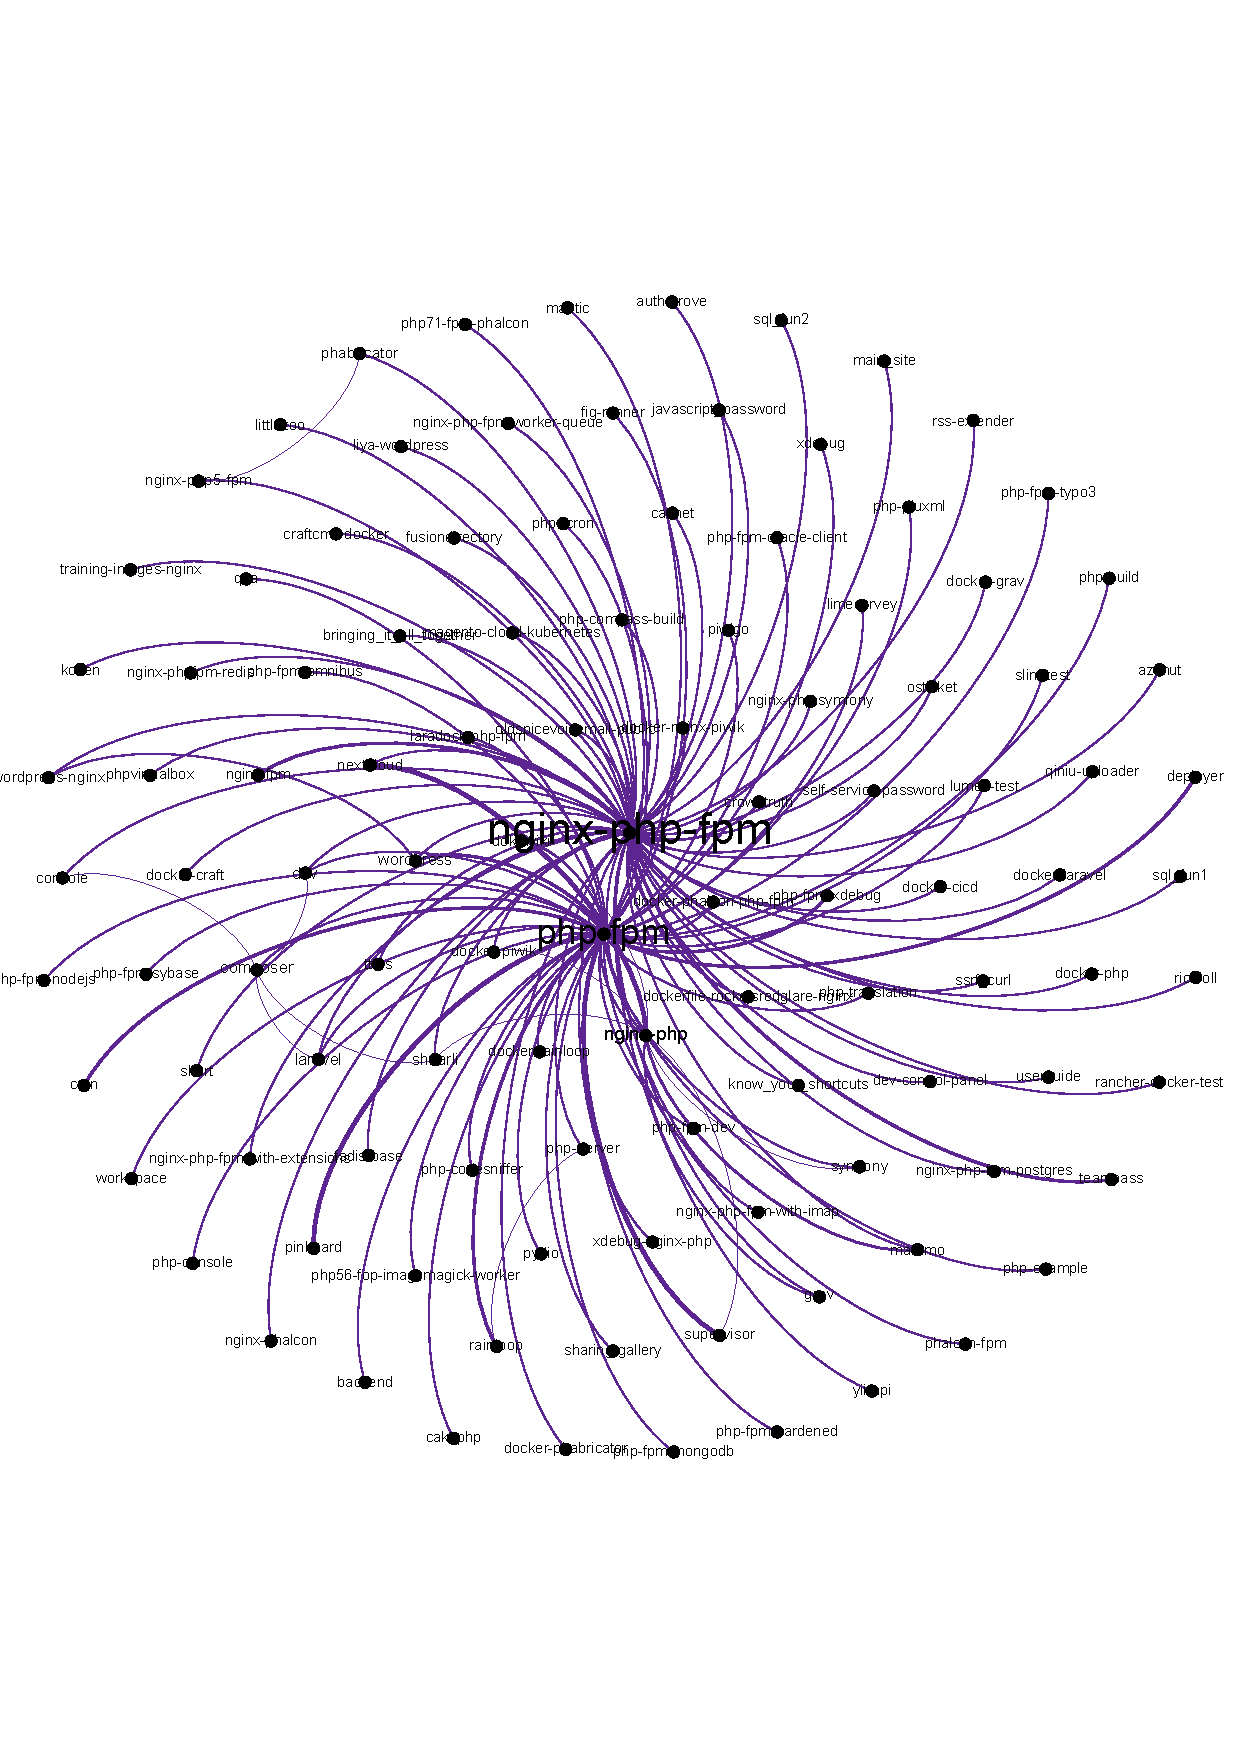
\includegraphics[width=0.35\textwidth,trim=10 130 10 %130,clip]{picture//image_network_pairs_nginx-php-fpm2.pdf}}
%\caption{The joint network of php-fpm and nginx-php-fpm.}
%\label{fig:php-fpm}
%\end{figure}


Those \emph{OS-OS} subnetworks can be understood as docker containers which can be built on several different types of operating systems and run successfully due to the common unix kernel of these distributed operating systems.  As for those \emph{OS-LR} subnetworks, docker containers are built based on the basic functions support of system software, such as scheduling tasks, executing applications, and controlling peripherals and meanwhile the support of programming language designed to work on a variety of platforms.  For those \emph{LR-LR} subnetworks, docker containers are built because of different function modules may be more appropriate to use different languages. %{\color{blue} Acturally, Many large-scale software development is not limited to one language. }  
For those \emph{OS-AF} and \emph{OS-TS} subnetworks, operating systems manages all of the other application programs in a computer and platforms or application can't run without support of \emph{OS}. %Thus, this relationship is not hard to understand. 
Interestingly, \emph{TS} or \emph{AF} subnetworks nearly didn't interact with the same type of subnetworks as oneself, however, they are relatively more inclined to interact with subnetworks whose type are \emph{OS} or \emph{LR}.   
A potential explanation is that \emph{TS} or \emph{AF} are inclined to implement a specific function or developed to a specific field, however, \emph{OS} and \emph{LR} provide more foundational aids for software development and thus what they oriented is the whole software ecosystem. Meanwhile, subnetworks of \emph{TS} or \emph{AF} are not completely independent, they also interactive for cooperation targets in a relatively infrequent way. %, e.g., Tomcat cooperates with Maven for realizing java web project, as shown in Figure~\ref{fig:maven-tomcat}.
%Based on the the subnetworks type count in TOP-100 and type feature ranked by linking strength, we consider relatively tight subnetworks pairs including OS-OS OS-LR LR-LR OS-TS and LR-TS OS-AF deserve further analysis and explaination. These mode are closely related to software evolution. 
%\noindent\textbf{OS-OS }  This paradigm can be understood as docker container can be built on several different types of operating systems and run successfully due to the common unix kernel of these distribution operating systems. For instance, even if a container built by centos container can also function as ubuntu kernel running on ubuntu operating system if the applications does not depend on the kernel. 
%\noindent\textbf{OS-LR }  In this paradigm, docker container are built based on the basic functions support of system software, such as scheduling tasks, executing applications, and controlling peripherals and meanwhile the support of programming language designed to work on a variety of platforms. Compared with other paradigms, the linking compansess of this paradigm is easiest to understand duo to the foundational aids of these two type containers. 
%\noindent\textbf{LR-LR }  In this paradigm, docker container are built because of different function modules may be more appropriate to use different languages. {\color{blue} Acturally, Many large-scale software development is not limited to one language. }
%\noindent\textbf{OS-TS }  In this paradigm, operating systems manages all of the other application programs in a computer and application/tools make use of the operating system. So the clostest linking to applications is that the operating system is not hard to understand.
%The reason may be that, on the one hand, ....  

After looking into the relationships between subnetworks, we find two common relationships:  %divide their relationships into three pattern: 
%\emph{Cooprative} and \emph{Alternative}.%, and inclusion relationship. 
(1) \noindent\emph{Cooperative relationship}: This pattern is particularly common in our dateset. %Detailed, 
Different types of containers solve different problems and domains so they always work together to accomplish complex functions. E.g., Tomcat cooperates with Maven to develop web pages, as shown in Figure~\ref{fig:maven-tomcat}.  %and PHP cooperates with ubuntu to provide basic system and language development environment. 
Also, some dockerfiles would have several FROM instructions at the same time,  %dockerfile will depend on two basic containers at the same time always suits the co-cooperate need for software development, 
e.g., the front-end development uses PHP as base image, while after-end development uses java. (2) 
% !!ubuntu_alpine  centos_debain     choose  one 
\emph{Alternative relationship}: This pattern is more easily seen between the same type of subnetworks. Some containers are dependent on different subnetworks in this pattern because they can realize function through any of the subnetworks due to the similar functions. The relationship between similar container subnetworks, thus, is considered as an alternative relationship.
Figure~\ref{fig:ubuntu_alpine} gives the joint network of ubuntu and alpine, which both can provide basic systems for other containers but differs in size and community support. 
%Figure~\ref{fig:centos-debain} gives a direct example of centos and debain, which both can provide basic systems for other containers but differs in size and community support.  
Significantly, reduce system size and runtime resource consumption accords with the lightweight technical feature of docker. The similarity between operating systems, additionally, can be applied to operating systems recommendations when building docker containers based on the principle of lightweight. 
 

%\noindent\textbf{Inclusion relationship} Relatively speaking, this pattern is not particularly common, but it is a product of adaptation to docker development. Some core containers are hard to define its type because of multiple attributes. This is because some containers are often combined to complete a complex functions, so the multi-attribute container has the significance of existence. For instance, to adapt the need of combining the php-fpm with nginx in one dockerfile for production deployment, core container nginx-php-fpm was created. Thus, the relationship between nginx-php-fpm and php-fpm can be identified as inclusion relationship showed in Figure~\ref{fig:php-fpm}. 



%A potential explanation is that 


\begin{mybox}
\emph{Answer to RQ6}: 
There is a correlation between the connection strength of the two subnetworks and their specific category groups. Particularly, the subnetworks in the \emph{OS-OS} group have higher inter-connection than other groups. 
Moreover, those linked subnetworks have cooperative or alternative relationship. 
%OS-OS OS-LR LR-LR OS-AF OS-TS has higher \emph{linking strength} indicating more reliable relationships while  TS-AF TS-TS AF AF are relatively more loose relationships. Cooprative, alternative and inclusion realitiobships between subnetworks promote jointlythe development of software in different ways.
\end{mybox}





\section{DISCUSSION}
\label{sec:di}
%Data collected from mobile phones have the potential to provide insight into the underlying 
%Every computer program, web application, and smartphone app has a creative mind behind it.

\subsection{Implication}
From our quantitative study results, we can distill some implications for different stakeholders.

\noindent\textbf{For researchers.}
The ability to automatically identify technical dependencies, generate subnetworks and character structure, diversity and relationship between subnetworks of docker containers opens the door for many interesting avenues of research: 

(1) \noindent\emph{Container summary generation}: There are more than 6 million  containers stored in the Docker Hub, having no tags or function descriptions is not conducive to understand or practical usage. Our construction of docker dependency network provides the feasibility of acquiring knowledge through configuration files. % Summary generation by 
Our instruction extraction and utilization of dockerfiles are conducive to automatic generation container summary. %Prior study on summary automatic generation of fork, code has have achieved performance. 

(2) \noindent\emph{Container recommendation}: We consider two kinds of recommendation applications for the docker containers. On the one hand, our empirical study finds alternative relationship between container subnetworks. It matters in size and build time when using alternative and lightweighter base image to build new container for software development,  especially for those large scale build applications. Thus, deeper studies on alternative relationship are needed for recommending automatically alternative containers. On the other hand, reliable dependency relationship between container networks can be captured from existing dockerfiles and give some related container recommendations. A series of recommendations for related containers may quickly help developers to understand this container from these cooperated or atterative containers.   

%Recommendation by function description


(3) \noindent\emph{Container version technical debt}: %Although we neglected the container version to highlight our research.   
In practice, a serious problem is the technical debt caused by the frequent changes of the container version. Our study reveals the function of the core container to improve software development and finds extremely popular OS containers that all identify their universal dependency relationship. Thus, impact on the whole docker ecosystem may be large if core container version changes. But how and even to what extent it influences to be further studied call the empirical on technical debt of docker container versions. 
Additionally, just-in-time recommendation of container version will also help to address this problem. 

%\noindent\textbf{container Tag recommendations} container tags can quickly help users to increase their understanding of containers, but in dockerhub, most private containers are lack of labels, which is not conducive to users' use of them. Our construction of container network and  research of container subnetworks relationship can help the container automatically generate descriptive tags, especially for the newly constructed container. 

(4) \noindent\emph{Container knowledge graph}: Our work mainly uses the base image to construct the container dependency networks. Researchers should integrate more dockerfile configuration data into this network, e.g., instruction complexity, container owner, project information, to form a container knowledge graph. Based on this knowledge graph, we can mine more knowledge and some patterns may become apparent. 



\smallskip
\noindent\textbf{For docker practitioners.} 
Our tools, constructing automatically subnetworks and subnetwork pairs of docker containers and further provide a visual presentation with the aid of Gephi engine. This way can give docker practitioners the most intuitive feeling from network angle about a given container and even multiple containers. Visual and direct tools may be a huge attraction to incoming docker practitioners who can access quickly the associated other containers, including connection relationships, and to what extent with the provided containers and even deepen the understanding of this container through the associated containers.     



\smallskip
\noindent\textbf{For tool builders.}
Our study finds that very few dominant containers have an obviously greater influence on the overall docker ecosystem. Tool support for effective and accurate containers tags and summary even maintenance of dominant containers may aid stronger docker ecosystem appeal. 
We also find that the strongest subnetwork pairs type is \emph{OS-OS} that indicates containers may have multiple alternative \emph{OS} base containers. Tools recommending as small as possible basic \emph{OS} containers under the premise of meeting the needs of developers will reduce build time in practice and in line with lightweight technical principles.  






\subsection{Threats To Validity}
\noindent\textbf{Threats to internal validity. }The threats to internal validity relate to errors in our experimental data, tool implementation, and personal bias in container classification. 
To avoid errors during the experiment, we carefully test our data processing tool and verify the accuracy of our tool implementation by manually examining a large number of data instances outputted by each step of our tool. To reduce the personal bias in container classification, two authors do this classification independently and the tiny difference comparison results show the reliability of our manual classification.    


\smallskip
\noindent\textbf{Threats to external validity. } One threat to validity is that our dataset consists of only 129,463 dockerfiles, the results may not be representative of all docker containers in Docker Hub. However, we make rigorous hypothesis tests on our analysis results. Besides, our approach capturing container pairs and constructing subnetworks hence can also be applied to other dockerfiles in Docker Hub.  
Another threat to validity is related to our selection of appropriate metrics to evaluate scale and interconnection in subnetworks, relationships between subnetworks. To mitigate this threat, we always use common and intuitive metrics and eliminate the unreasonable metrics through a large number of instances of visualization.   
  
% container versions 





\section{RELATED WORK}
\label{sec:rw}
\subsection{Docker and Dockerfiles}
%Docker build

%Dockerfile Smells 
With the increase in relevance of Container concepts, such as docker, 
empirical research on the Docker-based software development process has received more attention. Zhang et al.~\cite{zhang2018one} 
studied two prominent workflows, based on the automated builds feature on Docker Hub or Continuous Integration services, 
facing different trade-offs and this study further arises developers' focus on Docker-enabled workflows. 

To promote the application of containers, more research focuses on the evolutionary, 
configuration, and build-quality of containers. Wu et al.~\cite{wuempirical} conducted a large-scale 
empirical study of build failures including frequency, fix effort, and evolution in the Docker context, 
and pointed that the failure rate and fix time of Docker build fluctuate and gradually increase across time.
 A clustering-based approach for mining Dockefile evolutionary trajectories proposed by Zhang et al.~\cite{zhang2019clustering} 
 revealed six distinct clusters of Dockerfile evolutionary trajectories. Hassan et al.~\cite{hassan2018rudsea} proposed RUDSEA, 
 a novel approach to recommend updates of Dockerfiles to developers based on analyzing changes in software
  environment assumptions and their impacts.  %Dockerfiles smell Wu et al.


While the existing literature helps researchers and practitioners gain a deeper understanding of Dockerfile usage
and quality, few studies have investigated the docker container dependency,
the only exception being the study by Cito et al.~\cite{cito2017empirical}. In that
paper, the authors reported on an exploratory study with the
goal of characterizing the Docker ecosystem, prevalent quality
issues, and the evolution of Dockerfile. Their study was mainly
based on sampling inspections of Top-100 and Top-1,000 most
popular projects. Our work here is substantially different in
two aspects. First, we consider a more refined set of studied
dockerfiles, enabling powerful network construction and quantitative hypothesis testing, in addition to the basic statistics. 
Second,
our goal is different, as we aim to comprehensively understand
the characteristics, diversity, and relationship of the container dependency network.
%Jürgen Cito et al.\cite{cito2017empirical} studied Docker container type characteristics in Github, however, this study did not do a further discussion on the relationship between containers and the detailed differences between them. 




%Also, some studies investigated the tag recommendation approach of Dockerfile and the Dockerfile Temporary File (TF) smells. Specifically, Yin et al. [21] used Labeled Latent Dirichlet Allocation (LDA) algorithm to recommend tags,by taking a Dockerfile as the specific text description. Recently, Zhou et al. [22] proposed a semi-supervised learning based tag recommendation approach, SemiTagRec, for Docker repositories, and their results obtained good performance. As for the Dockerfile TF smells, Lu et al. [23] made an empirical case study to the real-world Dockerfiles on Docker Hub. They summarized four different patterns of TF smells and proposed a state-depend static analysis method to detect them. Further, Xu et al. [24] proposed two different methods to detect TF smells in Dockerfile with dynamic analysis and static analysis respectively. Experimental results showed that their methods perform effectively.



\subsection{Technical Dependency Network}
With projects are developed and co-evolve with each other, research emphasis of code repositories has 
shifted from single project to complex software ecosystems~\cite{zhang2018within}. 
The rise of technical dependency benefits from its ability to define ecosystem structure~\cite{lungu2010recovering}. 
Much work has been done studying software evolution, ecosystems 
by static analysis of the project configuration files~\cite{gonzalez2009macro,lungu2009reverse,santana2013towards}.  
Ossher et al.~\cite{ossher2010automated} proposed analyzing import statements in Java source code to recover dependencies 
between the software projects of an ecosystem. 
Alexandre Decan et al. carries out a quantitative empirical on package dependency networks for seven 
packaging ecosystems of varying sizes and 
dependency networks tend to grow over time, both in size and in number of package updates. 
Zimmerman et al.~\cite{zimmermann2008predicting}  have applied incorporating metrics that are based on the 
dependency graph of a software system to improve prediction performance and Nguyen et al.~\cite{nguyen2010studying} 
further studied the impact of dependency network measuring on software quality. They found that a small subset of 
dependency network measures have a large
impact on post-release failure. 
Blincoe et al.~\cite{blincoe2015ecosystems} proposed reference coupling method to establish technical dependencies 
and identify ecosystems using it.  



Despite the importance of docker in industry, to the best of our knowledge, no existing research has investigated the docker 
container from technical dependency network, nor empirically studied the structure, diversity, and relationship. 
With this paper, we attempt
to address this research gap and provide insights into the docker dependency management.


%For example, dependencies can be made available through a project’s configuration files, dependency manager files or through publicly available dependency specifications






\section{CONCLUSION}
\label{sec:co}
In order to better understand the dependency network of docker containers,
we construct the container dependency network from a set of more than 120,000 dockerfiles. We first investigate the characteristics of the container dependency network, including basic network metrics, degree distribution, and dominant containers. Next, for the Top-100 dominant containers, we construct their subnetworks and analyze the diversity and relationship among them. Our results help the researchers and practitioners gain a better understanding of the container dependency networks. 

In future work, we plan to build visualization tools for the container dependency network. Also, we plan to investigate the evolutionary characteristics of the container dependency network during different time periods. 

%Our method opens the door for future research in Dependency Network of Docker container including recommendation for associated containers, container version of technical debt etc. Our qualitative study results identifies that subnetworks of Docker core contain differ in structure and Interconnectness.    Our quantitative study results discovered and summarized relationships between sub-networks of docker containers.
%Our study sheds light on how Docker containers interact with each other to promote Dcoker ecosystem, and .

\section*{Acknowledgment}This work was supported in part by the National Key Research and Development Program of China (Grant No.2018YFB1004202), in part by the Foundation of PDL (Grant No.6142110190204), and in part by the Laboratory of Software Engineering for Complex Systems.


\bibliographystyle{plain}
\bibliography{ref}


\end{document}
\endinput
%%
%% End of file `sample-sigconf.tex'.
